\documentclass[12pt]{report}
\usepackage[a4paper, left=1in, right=1in, bottom=1in, top=1in]{geometry}
% install / use required packages
\usepackage{nomencl}
\usepackage{array}
\usepackage{mathtools}
\usepackage{nicefrac}
\usepackage{float}
\usepackage{subcaption}
\usepackage{adjustbox}

% \usepackage{chngcntr}
% \counterwithin*{equation}{chapter}
% \counterwithin*{equation}{section}
% \counterwithin*{equation}{subsection}

\usepackage{tikz}
\usetikzlibrary{shapes.geometric,arrows,calc}

\usepackage{caption}
\captionsetup{justification=raggedright,singlelinecheck=false}
\captionsetup[subfigure]{justification=centering}

\usepackage{graphicx}
\graphicspath{ {./images/} }

% \setcounter{tocdepth}{3}
\setcounter{secnumdepth}{4}

\title {
    THE IMPACT OF THE STORAGE FACILITY ON PERFOMANCE PARAMETERS OF AQUEOUS FILM-FORMING FIRE-FIGHTING FOAM (AFFF) IN AVIATION FIRE PROTECTION

    
\includegraphics[scale=1.5]{logo.png}
}
\author{Nhlanhla Fortune Khanyi}
\date{August 2022}

\begin{document}
\maketitle

\tableofcontents
\listoffigures
\listoftables

\nomenclature{P}{Pressure}
\printnomenclature

\makenomenclature

\chapter{Introduction}
This chapter provides an overview of the content structure of the study and the background of the issues underlying this study. The research objectives are comprehensively stated in accordance with the research outputs the study seeks to achieve. The motivations behind the present study are clearly stated. Moreover, an overview of the format/layout of the entire dissertation is briefly discussed and the content of the following chapter is stated. 

\section{Overview}
Airports Company South Africa (ACSA) is a main airport management enterprise in South Africa. ACSA was established in 1993 as a public company under the Airport Act (No. 44, 1993). Most of ACSA is owned by the South African government. Nevertheless, ACSA is active in commercial law. Over the years, the company has succeeded in providing a customer-oriented, commercially successful company whose airport has proven to be a symbolic and vital service element of South Africa. To date, ACSA owns and manages nine (9) South African airport communities in several provinces. As a state-owned enterprise, ACSA has an extra mandate to sincerely hand over profitability to its shareholders.
The company owns a number of assets that are critical thus should be effectively and efficiently maintained. As a consequence, ‘fire protection’ is a critical sector within any aviation industry, which has created divergent opinions in terms of compliance standards. Aircraft accidents are devastating, considering that loss of lives and costly equipment must be expected. In aviation, firefighting foam, particularly aqueous film-forming foam (AFFF) is a sole optimum extinguishing agent for suppression of combustible or flammable liquids. In South Africa, aviation accidents involving aircrafts have dramatically decreased over the past years. Nonetheless, it is obligatory for ACSA to adhere to the relevant compliance standards and be fully equipped in case of any unexpected circumstances.
Periodic training is mandatory in any aviation fire protection in ensuring that firefighting skills and resources within the sector adhere to the Federal Aviation Administration (FAA), National Aviation Authority (NAA), and National Fire Protection Association (NFPA) compliance standards, to react rapidly during accidents. Consequently, periodic testing of the performance parameters of fire extinguishing foam is a necessity. Unexpected circumstances often happen during periodic tests, when AFFF is unable to perform as anticipated. The main priority of AFFF is to suppress the fire and allow possible victims to have more time to escape during the accident. However, all this must be achieved in 1 minute or less upon the arrival on the accident scene, according to relevant compliance standards. The poor performance of AFFF is caused by numerous and diverse factors, hence it becomes difficult to examine where the problem originates.
In recent years, there have been fatal fire accidents in the aviation industry, which has tasked researchers to investigate further on the fire protection sector. Nevertheless, there are still notable gaps in previous research conducted, with limited studies on the impact of the storage tank of the firefighting foams. This is due to the nature and diversity of these problems. The complexity in focusing on the optimization of firefighting foam on the storage facility has always been a concern due to complicated branches of engineering such as material sciences, structural analysis, and thermal engineering involved. 
In 1965 Meldrum et al [1] published their study on storage life and utility of mechanical firefighting foam liquids. The study contributed to predicting the period in which firefighting foams can be held in a storage facility before they deteriorate. Furthermore, it emphasized the gaps and limitations within previous research and the difficulties in problem optimization. The predictions are governed by parameters such as extreme temperatures, oxidation, evaporation, corrosion, dilution, and contamination on the storage facility. Most of this research work will be benchmarked by [1], extensive research on the impact the storage facility has on AFFF will be conducted in various branches of engineering (material sciences, structural analysis, and thermal engineering).
This research work has a great significance in terms of evaluating the impact of storage facilities/tanks on AFFF performance, which is also dependent on a number of factors that have been previously stated. All manufacturers of firefighting foam concentrate have strict recommendations of storing their products, with the priority being to store foam concentrate in its original storage tank. The challenge rises due to critical factors that must be taken into consideration and often result to large storage tanks being constructed on-site. The large storages are beneficial as foam concentrate can be pumped rapidly from one source to firefighting vehicles during emergency conditions without the huge demand of replenishing. Consequently, these critical considerations lead to storing firefighting foam concentrate in different storage tanks rather than the recommended original containers.
 Motivated by these challenges, the purpose of the present research work is to experimentally evaluate and assess the impact of the materials utilised storage facility on the performance parameters of AFFF (state the exact parameters we are concerned with). The study examines the compatibility of engineering materials such as high density polyethylene (HDPE), mild steel and stainless steel. These are the materials that are commonly utilised when constructing a storage facility for firefighting concentrate, AFFF in particular. In this way, it is possible to enhance the properties of these engineering materials based on the heat treatment process, microstructural analysis, environmental stress cracking, and corrosion phenomenon. All these optimization methods are aiming to effectively store AFFF solution without the affection of the performance parameters and chemical composition during vital fire accidents. 

\section{Thesis layout}
The study consists of six chapters structured as follows:

\noindent \textbf{Chapter 1: Introduction} \\ 
This chapter provides a brief overview of the organisation included in the study as well as the background to the problem underlying the research work. It outlines the aim and the importance of the study. It explains the research objectives, formulates the research questions, and discusses the format of the study.

\noindent \textbf{Chapter 2: Literature review} \\
Chapter 2 provides a comprehensive summary of the existing literature on AFFF that was consulted. It focuses on the broader knowledge of previous studies that relate to the problems of interest in this study.

\noindent \textbf{Chapter 3: Evaluation of materials of construction} \\
The current and previous studies on the compatibility of engineering materials with AFFF concentrate is conducted. This is then validated by the experimental analysis in chapter 6 based on the outcomes.

\noindent \textbf{Chapter 4: Experimental set up} \\
The experimental set-up for the tests that were conducted in this study are documented in this chapter. All the materials and equipment used during the tests are also shown.

\noindent \textbf{Chapter 5: Results and discussion} \\
This chapter documents and discusses the results from the experimental tests in chapter 5. The results are compared between the various engineering materials. Results from other researchers are also compared with that found in this study. 

\noindent \textbf{Chapter 6: Conclusions and further work} \\
This chapter concludes the study with a summary of research findings aimed at solving the
research problem. The scope for future research areas is discussed and the conclusion for the entire study made.

\chapter{Literature review}
\section{Introduction}
This chapter aims to provide an overview and foundation of the current knowledge of this study in literature as well as a theoretical base for the work done in this study. Fundamentals pertaining to this study are presented. The solution techniques related to AFFF have been proposed and analysed by many researchers. All optimization problems are about maximizing the effectiveness and efficiency of AFFF. Inputs and outputs of these solution techniques have different limitations and difficulties which lead researchers to propose ideas about finding the best solution to these techniques.
The first section of the literature is a brief overview of significant fundamentals of AFFF- focusing on the evolutionary changes, characterization, foaming ability, mechanical stability, and critical application rates. This is followed by a review and analysis of current problems and difficulties based on the optimization of AFFF. Issues concerning the compatibility of various storage facilities on AFFF are discussed. Previous studies and experimental work aiming at the optimization of AFFF are discussed.

\section{A brief overview of various firefighting foams}
In the aviation industry, fire is of great concern due to the incidences of fires that are usually devastating to both human lives and properties. Since fire is of great significant in the present research, it is beneficial to understand various classes of fire. Fire is usually classified in five (5) classes. In fire science, fire is classified by the type of fuel they burn namely: Class A, B, C, D, and K. [2].  The classes are discussed in detail in Table \ref{ch2:table:classes}. However, the present research work will only focus on Class B fire, since AFFF is utilised to suppress this Class of fire.

\begin{table}[H]
\centering
\caption{Various classes of fire [3].}
\begin{tabular}{ m{.15\textwidth} m{.45\textwidth} m{.3\textwidth} }
\hline
Class of fire & Type of fire & commonly encountered \\ 
\hline
A & Common combustibles such as wood, paper, and rubber materials. & General places. \\
B & Flammable liquids such as fuel, petroleum greases, and flammable gases. & Airports and petroleum industries. \\
C & Energized electrical equipment and conductors. & Electrical distribution industries. \\
D & Combustible metals such as magnesium, titanium, and sodium. & Metal manufacturers. \\ 
K & Cooking oils, normal grease, and animal fat. & Production and FMCG industries. \\
\hline
\end{tabular}
\label{ch2:table:classes}
\end{table}

In the aviation industry, firefighting foam was declared by FAA as the sole optimal extinguishing medium used for suppression of Class B fire during emergency conditions. Originally, five types of firefighting foams are commonly used: fluoro protein foams (FPs), aqueous film-forming foams (AFFFs), film-forming fluoro protein foams (FFFPs), alcohol-resistant aqueous film-forming foams (AR-AFFFs) and alcohol-resistant film-forming fluoro protein foams (AR-AFFFPs) [4]. All of them were designed to be effective in handling precise fire conditions and contain one or more fluorinated surfactants as a key ingredient.
In general, foam is made by first mixing foam concentrate with water to create a foam solution. This aqueous solution is then blended with air using standard aspirating nozzles to generate foam [4].  Fire-fighting foam is an extinguishing agent composed of numerous bubbles formed mechanically or chemically from the liquid, as shown in Figure \ref{ch2:figure:scheme}. These are commonly used to reduce the spread and extinguishing of Class B fires and to prevent re-ignition whilst in certain situations may be implemented to extinguishing Class A fires [2]. Sometimes capabilities of firefighting foams can be reduced due to ignorance. Hence foam may be assumed to have performance concerns, whereas it does not. 

\begin{figure}[H]
    \centering
    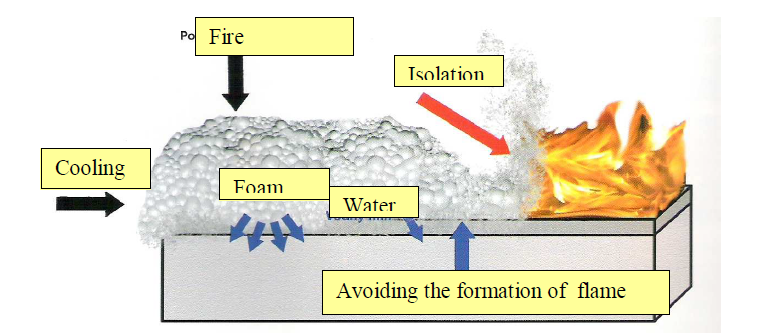
\includegraphics[width=.8\textwidth]{extinguishing_mechanism_scheme.png}
    \caption{Scheme of the extinguishing mechanism by using firefighting foam [5]}
    \label{ch2:figure:scheme}
\end{figure}

\section{Evolution of AFFF for effective extinguishment of Class B fires}
Water has long been a universal agent for suppression of fires, however, it is not exceptional in all instances [3]. For instance, water is regularly incapable of suppressing combustible fluids and can be perilous. Protein-based foams which presented a drastic improvement over water for combating liquid fuel fires were developed and used initially. These protein-based foams are thick and form a heavy, heat-resistant covering over a burning liquid surface [6]. These properties made protein-based foams to be constrained as they were not able to spread rapidly over the fuel surface. This was a concern for a long time, as protein-based foams were not much effective in low viscosity fuels such as kerosene that is commonly used in aviation industry. The ineffectiveness was due to the inability of protein-based foams to spread rapidly.
Synthetic based foams were developed and introduced in the mid-1960s to optimize protein-based foams [7] . These firefighting foams included AFFF and AR-AFFF. They generally provide better flow and spreading over the burning fuel surface, for faster knockdown of flames. AFFF concentrates are made from blending fluoro-and hydrocarbon-surfactant, modest quantities of salts and foam stabilizers are regularly included [8]. The AFFF concentrate is then mixed with a specific level of water to form a foam solution. The proportioning rate is usually, 1\%, 3\% and 6\% of foam concentrate to water. Furthermore, an additional feature of ‘aqueous film’ is formed on the surface of a flammable liquid by the foam solution as it drains from the foam blanket [3]. This film is very fluid and floats on the surface of most hydrocarbon fuels, hence providing AFFF with tremendous speed during extinguishing conditions. This made AFFF to be further developed and predominant to most firefighting foams. Moreover, the introduction of AFFF represented a significant increase in firefighting performance in terms of more rapid control and extinguishment of fuel fires, especial in industries that are involved with low viscosity fuels. The vital chemical composition of AFFF are depicted in Table A.1 on appendices.
It is essential to comprehend that Class B fires are exothermic reaction that relies significantly upon four (4) elements: fuel, air/oxygen, heat, and chemical chain reaction [9]. Removing one element will effectively halt the fire.  However, all firefighting foams do not interfere with the chemical reaction when extinguishing fuel fires, yet four (4) suppression mechanisms are required for knockdown and burn-back resistance:

\begin{itemize}
    \item The foam blankets the fuel surface smothering the fire. 
    \item The foam blanket separates the flames/ignition source from the fuel surface. 
    \item The foam cools the fuel and any adjacent metal surfaces. 
    \item The foam blanket suppresses the release of combustible fumes that can mix with air [9]. 
\end{itemize}

All firefighting foams were developed for suppression of specific combustible fuels. It is vital to identify which fuel group is involved when flammable fire conditions occur. This is to ensure timeous and effective extinguishment during fire conditions. As a consequent, firefighting foam may be ineffective when used on unsuitable fuel, hence may yield unexpected or unfavorable outcomes. There are two different basic flammable or combustible fuel groups:

\begin{itemize}
    \item Standard hydrocarbon fuels such as gasoline, diesel, kerosene, jet fuel etc. these fuels do not blend with water or are not miscible in water, they usually float on top of water and, for the most part, they do not intermix.
    \item Polar solvent or Alcohol type fuels are fuels that mix readily with water or are miscible in water [9].
\end{itemize}

To date, AFFF has been widely used in aviation fire protection for suppression of hydrocarbon fuels (a part of Class B fires). This synthetic based foam has a low viscosity and spreads quickly across the surface of most hydrocarbon fuels. Initially, AFFF was developed for aviation industries due to the fuel (kerosene) they are involved with and have proven to be effective in several cases. However, they can also be relatively utilized for extinguishing Class A fires. During firefighting a water film forms underneath the foam, which cools the liquid fuel, halting the formation of combustible fumes [6]. Consequently, this gives a sensational fire knockdown, which is a critical aspect in crash rescue firefighting.

\section{Foam generating process}
Foam, in general, is created by a mechanical action (dispensing equipment), hence the generation of firefighting foam is a mechanical process that comprises numerous prior steps. There are various methods of generating firefighting foam, each method relies on the class of fire involve and foam solution used. To date, there are three (3) methods of generating firefighting foam from a foam solution namely: aspirated nozzle, compressed air foam (CAF), and chemical reaction method [10]. The distinctions in these methods yield unique characteristics of foam produced with noticeable contrasts being the size and uniformity of the bubbles produced using each method [10]. Such differences may lead to significant variation of foam performance during fire conditions. However, the aspirated nozzle is a traditional and widely used method of generating firefighting foam, particularly in aviation fire protection.
Aviation fire protection have adopted the technique of aspirated nozzle when generating foam. This technique is more useful for aviation fire protection due to the type of environment and aviation standards that were developed and led by the National Fire Protection Association (NFPA). Technically and according to the research, the aspirated nozzle is suitable for low expansion foams such as AFFF and AR-AFFF [11].  Aviation fire protection utilizes AFFF for fire suppression due to the class of fuel (Jet A-1) they are involved with. Subsequently, the aspirated nozzle technique has been compatible with AFFF. However, during the periodic tests in aviation, the functionality of this technique is tested and according to the reports, there are still concerns when using it [10]. Moreover, the gaps exist in the optimization of this foam generation.
Comprehending of various foam generation methods is essential in the present research work in order to evaluate and deduce if any other method can yield any benefits. Most Research have been focusing on the aspirated nozzle and CAF generation methods aiming to optimize or implement new methods. Optimization of these methods require complex mathematical analysis as there are numerous parameters involved. Besides, the complexity further relies on the variation of chemicals involved in the chemical reaction technique.
In the present study, the aspirated nozzle technique is evaluated against CAF and chemical reaction methods in order to minimize or eliminate the optimization challenges of this foam generation method in aviation fire protection. The experimental work conducted by Laundess et al [10] shows that foam generated by CAF technique displays uniformly small size bubbles, aspirated nozzle produces a greater spread of bubble sizes while chemical (nitrogen) reaction displays most uniform size distribution of bubbles as shown in Figure \ref{ch2:figure:characteristics}. In addition, the CAF method has the advantage of being environmentally friendly.  With the aspirated nozzle technique having environmental concerns, a new technique or optimization has emerged as an alternative in aviation fire protection.

\begin{figure}[H]
    \centering
    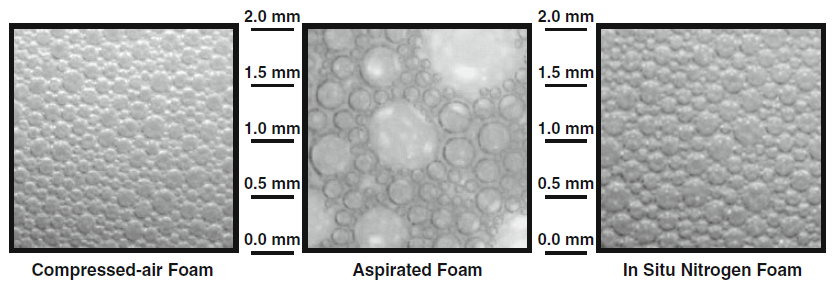
\includegraphics[width=.95\textwidth]{bubble_characteristics.png}
    \caption{Bubble characteristics for different generation methods [10].}
    \label{ch2:figure:characteristics}
\end{figure}

\subsection{Aspirated nozzle}
The technique has been extensively used and is the traditional way of generating firefighting foam. In this method, foam is generated by extracting air into a jet of foam solution inside a nozzle [11]. Most firefighting foam nozzles are specially designed in a convergent geometry. In this way, parameters such as pressure, velocity, and flow rate are carefully controlled as shown in Figure \ref{ch2:figure:nozzle}, foam solution at high pressure and low velocity enters the orifice at 1 and exit as finished foam at low pressure and high velocity at 5, at a constant flow rate. During stages 2, 3, and 4 air is drawn by a jet and blended with foam solution resulting in a strong mixing and agitation [12].

\begin{figure}[H]
    \centering
    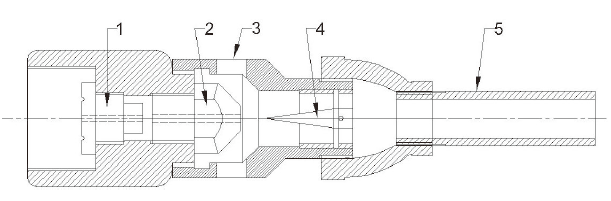
\includegraphics[width=\textwidth]{foam_generating_nozzle.png}
    \caption{Nozzle for generating foam [12].}
    \label{ch2:figure:nozzle}
\end{figure}

The governing equation for critical parameters during the foam generation is usually the Bernoulli’s equation, which is given as:

\begin{equation}
    P_1+\frac{1}{2}\rho{v_1}^2 + \rho gh_1 = P_5+\frac{1}{2}\rho{v_5}^2 + \rho gh_5
\end{equation}

As seen in Figure \ref{ch2:figure:nozzle}, in case where the potential energy at the elevation 1 ($\rho gh_1$) equals the potential energy at elevation 2 ($\rho gh_5$), then the equation can be simplified and written as:

\begin{equation}
    P_1+\frac{1}{2}\rho{v_1}^2 = P_5+\frac{1}{2}\rho{v_5}^2
\end{equation}

\noindent Where, \\
$p_1\ is\ the\ pressure\ at\ elevation\ 1\ in\ Pa$ \\
$v_1\ is\ the\ velocity\ at\ elevation\ 1\ in\ m/s$ \\
$h_1\ is\ the\ height\ at\ elavation\ 1\ in\ m$ \\
$P_5\ is\ the\ pressure\ at\ elavation\ 2\ in\ Pa$ \\
$v_5\ is\ the velocity\ at\ elavation\ 2\ in\ m/s$ \\
$h_5\ is\ the\ height\ at\ elevation\ 2\ in\ m$ \\
$g\ is\ the\ acceleration\ due\ to\ gravity\ in\ m/s^2$ \\
$\rho\ is\ the\ density\ of\ fuid\ in\ kg/m^3$ \\

Since convergent nozzles are used to increase the outlet velocity ($v_5$  in figure \ref{ch2:figure:nozzle}) due to the conservation of mass, while critically maintaining the inlet flowrate during firefighting. Therefore, the following assumptions can be made:

\begin{gather*}
    A_1 > A_5 \\
    V_1 > V_5 \\
    P_1 > P_5
\end{gather*}

When the areas of the inlet and outlet are known and the flow rate that must be achieved is also known, then velocities can be calculated using the following equation:

\begin{equation}
    Q = VA
\end{equation}

\noindent Where,\\
$Q\ is\ the\ flowrate\ in m^3/s$ \\
$V\ is\ the\ velocity\ of\ foam\ solution in m/s$ \\
$A\ is\ the\ area\ of\ the\ nozzle\ at\ a\ particular\ point\ in\ m^2$ \\

Over the years, researchers have been focusing on the source of these problems in order to comprehend the mathematical difficulties involved. However, engineers have been working on mathematical solution techniques in order to optimize convergent foam nozzles in aviation fire protection. Aspirated nozzle problems are noticeable during periodic trainings and uncertainty in the origination of the problem is mostly the challenge for many researchers.

\subsection{Compressed air foam (CAF)}
The CAF method is commonly used for generating any kind of firefighting foam and was developed initially by the National Research Centre of Canada (NRCC) in the late 1990s [13]. The technique has offered several benefits in fire protection since the prohibition of halogen-based agents due to some environmental impacts.  
CAF technique is similar to the aspirated nozzle method as it also consists of a divergent nozzle for discharging foam. The distinction is that, in the CAF system, air is pressurized using an air compressor then fed or injected in an aqueous foam solution, as the foam expands its then discharges and guided through a nozzle.

\subsection{Chemical reaction}
This is a modern technique that was discovered by [10] to eliminate foam generation problems. The method has not yet been recognized in fire protection standards but certainly has several benefits. With other generation methods extensively used to produce much heavier carbon dioxide bubbles, it was of great practical significance to evaluate other methods that will produce lighter uniform bubbles. Consequently, nitrogen gas bubbles were the empirical and realistic alternative. In this way, the chemical reaction of foam solution and nitrogen creates numerous, uniformly sized bubbles of nitrogen gas within the foam.
The method has been reviewed by many researchers.  The only concern is the need to optimize foam formulations to prevent surfactants from being affected by the nitrogen generation and by the presence of salts formed during chemical reaction [10].  For this reason, aviation fire protection will need to examine this as an alternative of possibly eliminating the aspirated nozzle method.

\section{Foaming ability and Mechanical stability}
Modern firefighting foams are primarily of the mechanical type. This means that before being utilized, they should be proportioned (mixed with water) and aerated (blended with air). Four elements are necessary to produce a quality and stable foam blanket and they include: foam concentrate, water, air, and aeration (mechanical agitation) [2].
In recent years, mechanical stability has been a concern for most firefighting foams. Many researchers have approached this challenge with the aim of optimization. Foaming ability is a key process in advancing the mechanical stability of firefighting foams. Foam is a collection of air bubbles produced from a foaming solution [2]. The rate of this transformation is essential for evaluating the mechanical stability of the foam. Stability properties, as well as the effectiveness of firefighting foams, are determined by their physical and chemical properties, as described by Turekova and Balog [5]. These properties may include: the number of foaming, viscosity, foam frost resistance, the content of the sediment, foam stability, half-life of foam, pH, foaming solution of spreading factor [5].
Synthetic based foams are low viscosity foams, consequently, they spread easily on the surface of the flammable liquid. This enables the formation of a dense and stable foam layer that acts as a physical boundary against the heat and mass transfer, thus exhibiting excellent cooling and covering effects in hydrocarbon fires [14]. The mechanical stability of AFFF depends upon the structure of surface films from the so called-foaming agents. During firefighting conditions, the foams are continuously disrupted by the influence of heat of ignition, the internal force of foam, and the hot surface of burning liquid [5]. Foaming ability is thus a fundamental procedure as it directly affects the quality, hence the performance of the foam. The important parameters affecting a foam's ability to extinguish hydrocarbon fuel fire was addressed by Joseph et al [6] as shown in Figure \ref{ch2:figure:parameters}, with a theoretical modeling to further evaluate the challenges and limitation of the current methods used. 

\begin{figure}[H]
    \centering
    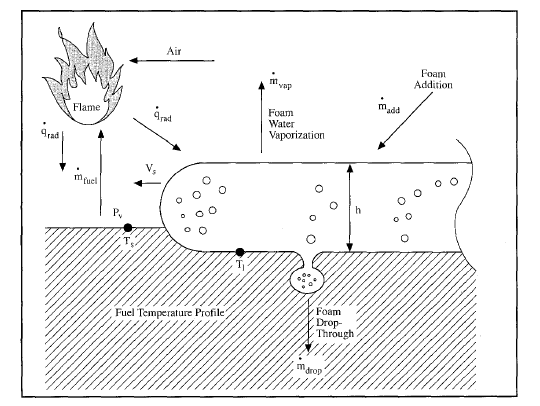
\includegraphics[width=\textwidth]{important_parameters.png}
    \caption{Important parameters affecting a foam's ability to exthinguishh hydrocarbon fuel fire [6].}
    \label{ch2:figure:parameters}
\end{figure}

Oguike [2] conducted experimental tests intending to assess the foaming ability of various foams. The analysis comprised of eight (8) empty bottles, different volume of water was added and a constant foam concentrate was also added. The bottles were shaken vigorously at a steady time in each case and foam height was recorded. The foams were left to stand for some time and heights were measured again. Foams were left to stand for further days and height was measured again. Finally, foams formed were left to stand until collapse, and time was recorded for each foam solution. This experiment set a benchmark for most researchers, as most of the other foaming ability experiments have been based on it.
The current challenge is to develop small-scale test methods that measure these parameters in such a way that they can be used to predict large-scale foam performance. Persson [15] described optimization techniques and results to investigate foam mass loss by evaporation as a function of radiant heat from a fire. The finding was that foam viscosity and spreading is an area requiring further investigation. 

\subsection{AFFF blanket stability/drainage time}
Drainage time is often used to analyze the stability of various foams, however, it does not provide a reliable indication of the firefighting capability of foams. Drainage time is a measurement of the rate at which foam solution drains out of finished foam and hence provides an indication of the stability of the foam blanket [7]. High expansion foams usually maintain the stability and heat resistance due to their long drainage time and hence slow loss of water from the finished foam. 
Since AFFF is a low expansion foam, there are difficulties in maintaining the stability and heat resistance from the finished foam. This is due to short drainage time which indicates that finished foam losses its water content rapidly and renders it vulnerable to high-temperature flames and hot surfaces. A basic principle of measuring low expansion foam expansion ratios is shown in Figure \ref{ch2:figure:tests}. In recent years, most researchers concluded that the drainage times of finished foams do not solely depend on foam concentrate but also the type of foam generation [16]. In most cases, drainage time for low expansion foams such as AFFF is often expressed as 25\% drainage time, while for medium and high it’s usually 50\% drainage time. This is the time taken for 25\% or 50\% of the original foam solution content (by volume) to drain from the finished foam, as shown in Figure \ref{ch2:figure:tests}.

\begin{figure}[H]

\centering
\begin{subfigure}{.45\textwidth}
    \centering
    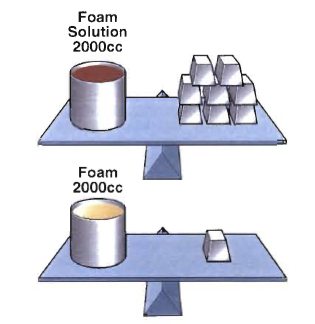
\includegraphics[width=\textwidth]{low_expansion_test.png}
    \caption{}
\end{subfigure}
\begin{subfigure}{.45\textwidth}
    \centering
    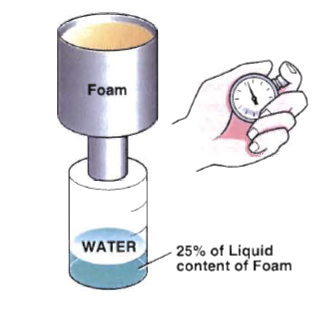
\includegraphics[width=\textwidth]{drainage_test.png}
    \caption{}
\end{subfigure}

\caption{a) Low expansion test and b) drainage test [7].}
\label{ch2:figure:tests}
\end{figure}

Researchers have been working on optimizing the foaming ability, hence the stability of foams, particularly for low expansion foams.  An experimental work to analyze and compare the drainage time and bubble size distribution of various firefighting foams was described by Mark et al [10]. Table \ref{ch2:table:times} shows the results of [10] comparing the 25\% of drainage times at an expansion ratio of 7:1 for two (2) different foam concentrates. \\

\begin{table}[H]
\caption{Comparison of 25\% drainage times at 7:1 expansion [10].}   

\centering
\begin{tabular}{m{5em} m{5em} m{4em} m{4em} m{4em} m{5em}}
    \hline
    & & & & 25\% Drainage time (s) \\
    \hline
    Foam concentrate & Generation system & Mean & Max & Min & Standard Deviation \\ 
    Tolomet 6\% & ISNF & 342 & 450 & 264 & 93 \\
    & CAF & 488 & 533 & 430 & 53 \\
    & Aspirated & 197 & N/A & N/A & N/A \\
    FC-600 3\% & ISNF & 539 & 725 & 450 & 126 \\
    & CAF & 1060 & 1281 & 844 & 288 \\
    & Aspirated & 485 & N/A & N/A & N/A \\
    \hline
\end{tabular}

\label{ch2:table:times}
\end{table}

The results indicate that drainage rates for the various foam types were quite different, which may be explained by differences in the bubble size distributions as discussed below in Figure \ref{ch2:figure:distributions}. To explain the differences in foam drainage rates between the three foam types, they studied the bubble size distributions for each foam type.

\begin{figure}[H]
    \centering
    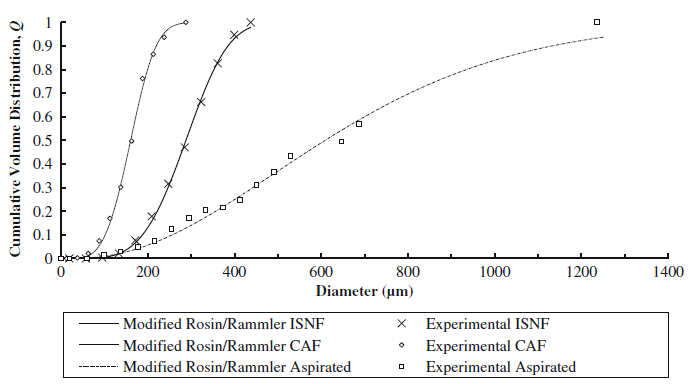
\includegraphics[width=\textwidth]{bubble_size_distributions.png}
    \caption{Cumulative bubble size distributions for various foam generation methods}
    \label{ch2:figure:distributions}
\end{figure}

As shown in Figure \ref{ch2:figure:distributions}, the drainage time is profoundly dependent upon the foam generation type. Also, the aspirated foam generation method produced larger bubbles in terms of size. These bubbles contributed to shorter drainage times as seen in Table \ref{ch2:table:times}, hence the reduction of foam quality and stability. This correlation technique used was benchmarked by [2] and most researchers have concluded the same as [10]. Mukunda and Dixit [12] constructed a model of foam drainage based on momentum flux balance and conducted experiments with an apparatus with foam drainage through a fuel layer. Their results showed a linear relationship of 25\% drainage time with the height consistent with the theoretical expectations. A recommendation made by [10] indicates that there is a need for further research to develop a new surfactant formulations immune to the oxidation reaction that generates nitrogen bubbles. This foam generation method will simultaneously increase the drainage rates and stability of low expansion foams due to nitrogen bubbles.

\section{Critical application rates}
In the most recent decade, most researchers have been interested in the application rates of various firefighting foams. A number of studies on effective application rates have increased significantly and most of these studies have been based on protein and synthetic based foams. The underlying motivation for considering diverse critical application rates was to identify the compatibility of foams on various class of fires. With the original motivation behind the development of synthetic based foams being economic issues, the application rates were, thus critical.
Most of the research on firefighting foams are based on optimization aiming to provide the necessary effectiveness and efficiency in performance. The basis for the current minimum application rates was originally developed in 1972 by Geyer [17] in tests of protein and AFFF solutions. These were "modelling" tests with jet propellant (JP-4) pool fires that measured 21 m, 30 m, and 43 m in diameter. They also included large-scale verification tests with a B-47 aircraft and simulated shielded fires, conducted with JP-4 pool fires 34 m and 43 in diameter with all tests conducted using air-aspirating foam generation method. The outcomes by [17] showed that PF and AFFF have an application rate with a ratio of 1.49:1 respectively and is shown in Figure \ref{ch2:figure:pool}. This difference in application rate recognizes the inherent advantage of using AFFF to extinguish hydrocarbon pool fires and reflects the fact that AFFF has been demonstrated to extinguish pool fires more rapidly than PF at equivalent application rates. For equivalent extinguishment times, lower rates of AFFF than PF are required [6].

\begin{figure}[H]
    \centering
    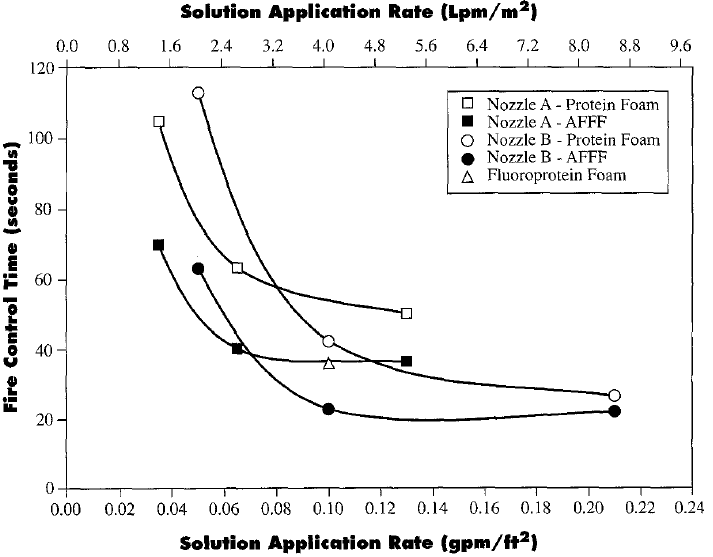
\includegraphics[width=\textwidth]{fire_control_time_pool_fires.png}
    \caption{Fire control time as a function of solution application rate using protein foam and AFFF on JP-4 pool fires [17].}
    \label{ch2:figure:pool}
\end{figure}

Numerous experimental tests have been conducted by many researchers with purpose of validating these application rates. Geyer et al [18] further conducted tests on critical application rates for validation. The experimental tests conducted were focused on fire control time as a function of solution application rate for PF, AFF, and FPF for Jet A fuel fires and the results are shown in Figure \ref{ch2:figure:fuel}. These were aiming in employing more foam generation methods and different fire type to make necessary analyses of outcomes and compare with [17]. Based on Figure \ref{ch2:figure:pool} and \ref{ch2:figure:fuel}, the application rate is greatly dependent on the type of foam generation and also the type of foam concentrates utilised. There have been numerous challenges regarding the critical applications of firefighting foams. The proliferation of performance guidelines and specifications for firefighting foams has created divergent opinions especially on aviation industry fire protection standards [6].

\begin{figure}[H]
    \centering
    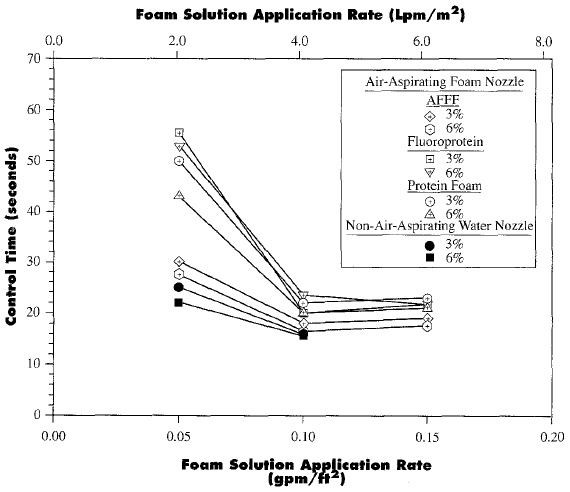
\includegraphics[width=\textwidth]{fire_control_time_fuel_fires.png}
    \caption{Fire control time as a function of solution application rate for AFFF, fluoroprotein and protein foams for Jet A fuel fires [17].}
    \label{ch2:figure:fuel}
\end{figure}

\section{Effect of degradability}
Aircraft accidents are currently not a threatening issue in South Africa. This is due to a drastic decrease in air-crash over the past years. Nevertheless, fire protection in South African aviation has always been compliant. Due to this drastic decrease in air-crash, firefighting resources including firefighting foam last a long time without actually being realistically tested. Firefighting foams naturally degrade over time due to several factors such as liquid drainage driven by gravity and coarsening. Firefighting foam degradation is defined by Hinnant et al [19] as a reduction in foam layer thickness regardless of any changes in foam density or ‘quality’.
In the present research work, it is essential to comprehend the impact of different storage facilities on foam degradation. In this way, advancing the storage facility focusing on degradation will be uncomplicated. Aviation periodic training is the only platform of testing foam performance parameters, hence foam degradation. As a result, it may not indicate the precise causes of degradation as this is not an actual situation. Foam’s effectiveness can be severely deteriorated by foam degradation. Thus, foam degradation can be influenced by many factors including the hot fuel, fire, and foam formulation that contains surfactants and additives needed to generate the foam [19]. Although these factors are known, some of them such as fuel and fire cannot easily be controlled.    
During the firefighting process, foam is continuously interacting with fuel and flame. The interaction may immensely destroy the thick layer of the foam [20]. In this way, the ability of foam will be reduced, thus its performance may be compromised. However, foam degradation may suddenly increase dramatically during this process.  The causes for this are not well understood due to the lack of research on foam degradation. Furthermore, the individual effect of fire and fuel on degradation are inseparable due to the presence of fire [19]. 
Previous research on foam degradation has mostly focused on the natural aging process of foam [21] and the effect of the interaction of hydrocarbon liquids with foam [20].  The natural aging of foam can be mainly influenced by the storage tank utilized, which is essential in this research work as the optimization of the storage facility based on degradation will be benchmarked by these previous Research. Hinnant et [19] studied the influence of fuel on foam degradation for fluorinated and fluorine-free foams. The study outcome showed that the fuel temperature is by far the major factor contributing to foam degradation followed by the effects of surfactant formulation, type of fuel, and bubble diameter or expansion ratio. Figure \ref{ch2:figure:degradation} shows the percentage change in AFFF thickness versus time at room temperature, 35, 50, 75, and 90℃.

\begin{figure}[H]
    \centering
    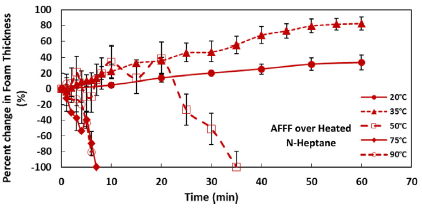
\includegraphics[width=\textwidth]{foam_degradation.png}
    \caption{AFFF foam degradation versus time over n-heptane fuel at different temperatures [19].}
    \label{ch2:figure:degradation}
\end{figure}

Parameters such as bubble diameter or expansion ratio are much dependent on the foam generation method, which is discussed in section 2.4. Larger bubbles cause a rapid drainage rate than smaller bubbles, and according to [19], the increased drainage rate can cause the foam to degrade rapidly. In this way, the storage facility may indirectly affect foam degradation. This is due to the sediments or sludge, which may accumulate in the storage facility during the aging process. Consequently, sediments may affect foam characteristics, particularly bubble distribution during the foam generation process, this is shown by employing a flow process in Figure \ref{ch2:figure:effect}. The optimization of a storage facility in reducing the accumulation of sediments will prove to extensively reduce foam degradation.

\begin{figure}[H]

\centering
\begin{adjustbox}{center}
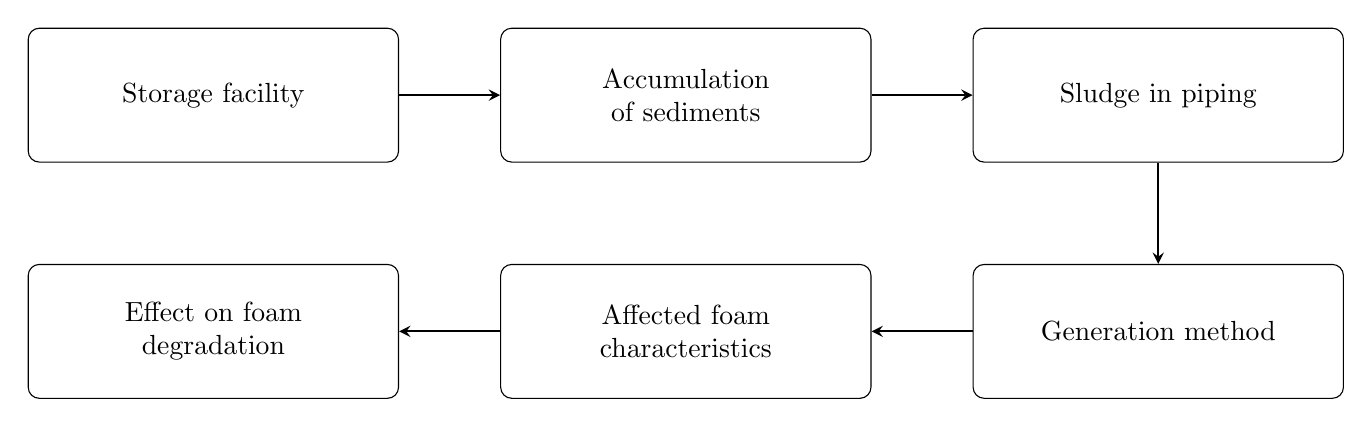
\begin{tikzpicture}[node distance=6cm]
    \tikzstyle{block} = [rectangle, rounded corners, draw, text centered, text width=4cm, inner sep=1em, minimum height=1.7cm]
    \tikzstyle{arrow} = [thick,->,>=stealth]

    \node (storage) [block] {Storage facility};
    \node (accumulation) [block, right of=storage] {Accumulation of sediments};
    \node (sludge) [block, right of=accumulation] {Sludge in piping};
    \node (generation) [block, below of=sludge, yshift=3cm] {Generation method};
    \node (affect) [block, left of=generation]{Affected foam characteristics};
    \node (effect) [block, left of=affect] {Effect on foam degradation};

    \draw [arrow] (storage) -- (accumulation);
    \draw [arrow] (accumulation) -- (sludge);
    \draw [arrow] (sludge) -- (generation);
    \draw [arrow] (generation) -- (affect);
    \draw [arrow] (affect) -- (effect);
\end{tikzpicture}
\end{adjustbox}

\caption{Effect of AFFF degradation.}
\label{ch2:figure:effect}
\end{figure}

There have been fewer studies on the effect of surfactant formulation on degradation, further research should be conducted to detect the effect of this parameter on foam degradation. Furthermore, other parameters that may affect foam degradation should be extensively investigated in the future as foam degradation may regularly affect the performance of the foam.

\section{Environmental issues}
Modern firefighting foams can be considered as sensational in terms of physical characteristics, but, in recent years, the new Registration Evaluation Authorization and Restriction of Chemicals (REACH) legislation have drawn attention to their ecotoxicological properties [5]. While AFFF is the most widely used firefighting foam in aviation fire protection, it still has some disadvantages, of which one of those is the environmental impact [22]. Due to growing concerns regarding the impact that firefighting foams have on the environment, steps need to be taken to rectify this situation. To date, few papers have looked at the environmental impact of AFFF. This lack of research on environmentally friendly surfactants must be addressed with more experimental studies to reduce the contamination of the environment, especially in aviation industry.
Although AFFF has numerous advantages over other firefighting foams, their environmental issues have been a huge setback. Initially, AFFF contained substances such as perfluoroalkyl and poly-fluoroalkyl (PFAS). Previous research shows that PFAS had significantly caused the contamination of soil, groundwater, and surface water including water stream animals as a result of AFFF being released during aviation periodic training [23]. As shown in Figure \ref{ch2:figure:use}, this poses acts of negligence and is hazardous to the environment as foam detoxifies naturally in soil.

\begin{figure}[H]
    \centering
    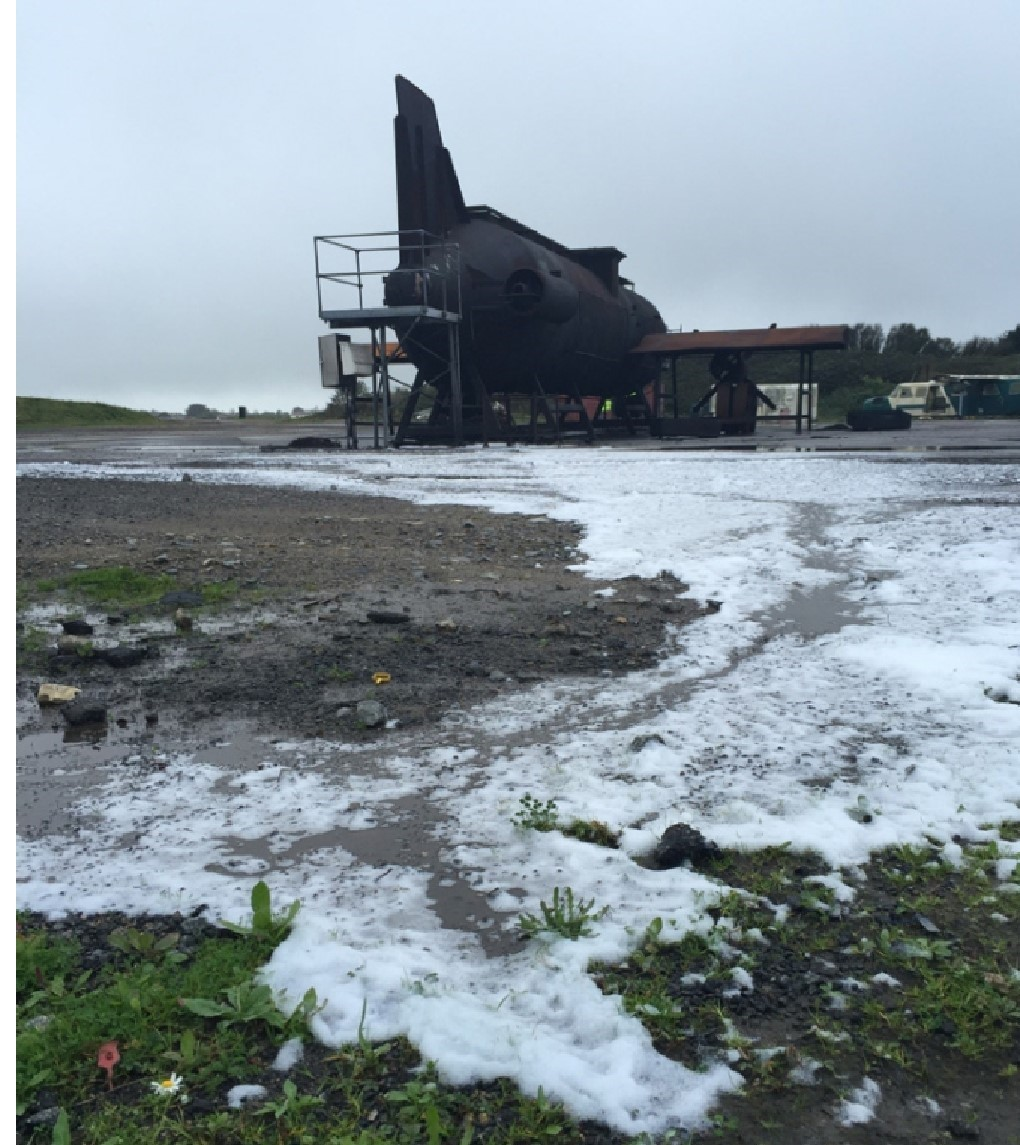
\includegraphics[width=\textwidth,height=9cm]{use_during_aviation_training.jpg}
    \caption{Used AFFF during aviation periodic training.}
    \label{ch2:figure:use}
\end{figure}

Initially, PFAS's have not been previously known or recognized to be harmful in the environment. This was due to the complexity of AFFF mixtures utilized and previous significant gaps in thorough comprehending of PFAS, including their toxicity, bioaccumulation, occurrence, transport, and transformation mechanisms [23]. However, PFAS's impact in the environment was then recognized in the late 1990s and several jurisdictions offered guidance with a limited range or amount of PFAS's that can impact the environment [19].
Elimination of PFAS in AFFF was a challenge for every manufacturer and aviation industries as these chemical substances were key during fire suppression. AFFF was able to suppress fire rapidly due to the presence of PFAS's. With environmental regulations enforcing the elimination of PFAS, manufacturers had no other alternative but to cooperate in the elimination of PFAS's. Consequently, PFAS's were phased out in 2002 by all the manufacturers due to the environmental impact [24].  Fluorinated surfactants replaced PFAS's instantly intending to reduce the environmental impact and still be compatible with AFFF. 
According to the research, fluorinated surfactants were also found to have an impact on the environment [16]. As a result, samples that were analyzed in 2010 indicate that AFFF manufacturers have commenced to gradually reduce or even eliminate fluorinated surfactants in their formulations [23]. Moreover, this process of eliminating present surfactants is critical as the transition should be carefully analyzed, in order to prevent the possible negative influence, it might pose in the performance parameters of firefighting foam. To date, fluorinated surfactants are present in AFFF and are continuously bio-persistent in the environment and pose health hazards to humans.
The main objective of the present research work is to improve the compatibility of the materials that are utilised to construct the storage facility. Therefore, the environmental issues of AFFF are of significance in the present study, since the optimised storage materials should not negatively influence the composition of AFFF, as this might then cause environmental issues during firefighting. 
In recent years, researchers have been investigating the effective ways of mitigating the environmental issues. While the progress of this optimization has been held back by the difficulties stated above. The NFPA committee, which is responsible for NFPA 11, low expansion foams, has made significant effort in tasking a group to address the environmental concerns around low expansion foams [6]. The outcome of the task group has been recently published with a full guidance to end user[6]. Alternatively, researchers have managed to implement new surfactants which are environmentally friendly. However, commercial firefighting foams without fluorinated surfactants developed to date have not been able to extinguish the fire as rapid as AFFF [19]. In the future, researchers will need to conduct an extensive investigation in order to implement the environmentally friendly surfactants that will be compatible with AFFF.  

\section{Conclusions}
This chapter reviewed the relevant literature to gain a better and in-depth understanding of the various firefighting foams. The focus was diverted to AFFF, where the evolution of this type of foam was studied. Various foam generation processes were discussed, and their impacts on the poor performance of AFFF. Based on the previous studies, the aspirated nozzle is suitable for generating AFFF. The equations involved during this process were analyzed, with some recommendations to optimize this process being detailed. The importance of the foaming ability and mechanical stability were addressed, and the findings of previous studies were discussed. It was then found that the stability directly affects the quality, hence the performance of the foam.
The drainage time of AFFF was evaluated, this was based on the previous experimental work. It is concluded by many researchers that AFFF has a short drainage time which indicates that finished foam losses its water content rapidly and renders it vulnerable to high-temperature flames and hot surfaces.
The critical rate at which AFFF should be applied was another key factor in this chapter. Not many researchers have succeeded in determining these critical rates. Consequently, some of the performance guidelines and specifications for firefighting foams have created divergent opinions, especially on the aviation industry. The degradation of AFFF concentrate was another discussion. It was found that the increase in the degradation may immensely impact the performance of AFFF. The causes for the increase of degradation are not well understood, due to the lack of research on foam degradation. This chapter concluded by addressing the environmental issues of AFFF. Numerous researchers have investigated effective ways of mitigating these environmental issues. Implementation of environmental surfactants was a recommendation of many researchers.
The next chapter evaluates the various engineering materials commonly used to construct the storage facility for AFFF concentrate. It further investigates and recommends possible ways of enhancing the properties of these materials based on the current knowledge.

\chapter{Evaluation of materials of construction}
\section{Introduction}
This chapter details an in-depth understanding of the engineering materials commonly used to construct the storage facility for AFFF concentrate. The scope of this chapter includes a brief overview of these materials to thoroughly understand how they are classified. It further details the properties of interest for each material and why they opted as storage facilities.
Fundamental literature concerning the evolution of these materials is detailed in this chapter. The corrosion phenomenon is investigated in each material to understand its effect on the performance parameters of AFFF. Furthermore, the understanding of the metallic bonding and cross-linking of these materials is vital. This is briefly discussed in this chapter. To improve the properties of these materials, the microstructure morphology must be better understood. This also aided when analyzing the microstructure of each material in chapter 6. In this way, is possible to optimize these materials once the metallic bonding, cross-linking, useful properties, and microstructure are well comprehended. Subsequently, the heat treatment processes are evaluated to make an effort of optimizing these engineering materials.

\section{A brief overview of construction materials}
As the economy becomes increasingly global, so the importance of materials increases. Storage facilities/tanks can be constructed using a variety of materials. The selection of the material can be a challenging systematic process that is commonly dependent on cost, reliability, availability, ease of fabrication, material properties, and environmental impacts [25].  The main goal to be achieved in this process being to minimize the cost while meeting the product performance, efficiently. However, for storage facilities, it may largely depend on the type of product to be stored. The product to be stored may vary in the state or phase of matter, which is critical to evaluate before any process commences. To date, there are five (5) different state of matter that are known: solids, liquids, gases, plasma, and Bose-Einsten condensate [26]. 
For the purpose of the present research work, the evaluation of the construction material will focus on the liquid state, since AFFF concentrate is in liquid form. In this way, the material that will be used to construct the storage facility can be significantly evaluated. The classification of engineering materials is shown in the form of a flow chart in Figure \ref{ch3:figure:materials}.

\begin{figure}[H]
    \centering
    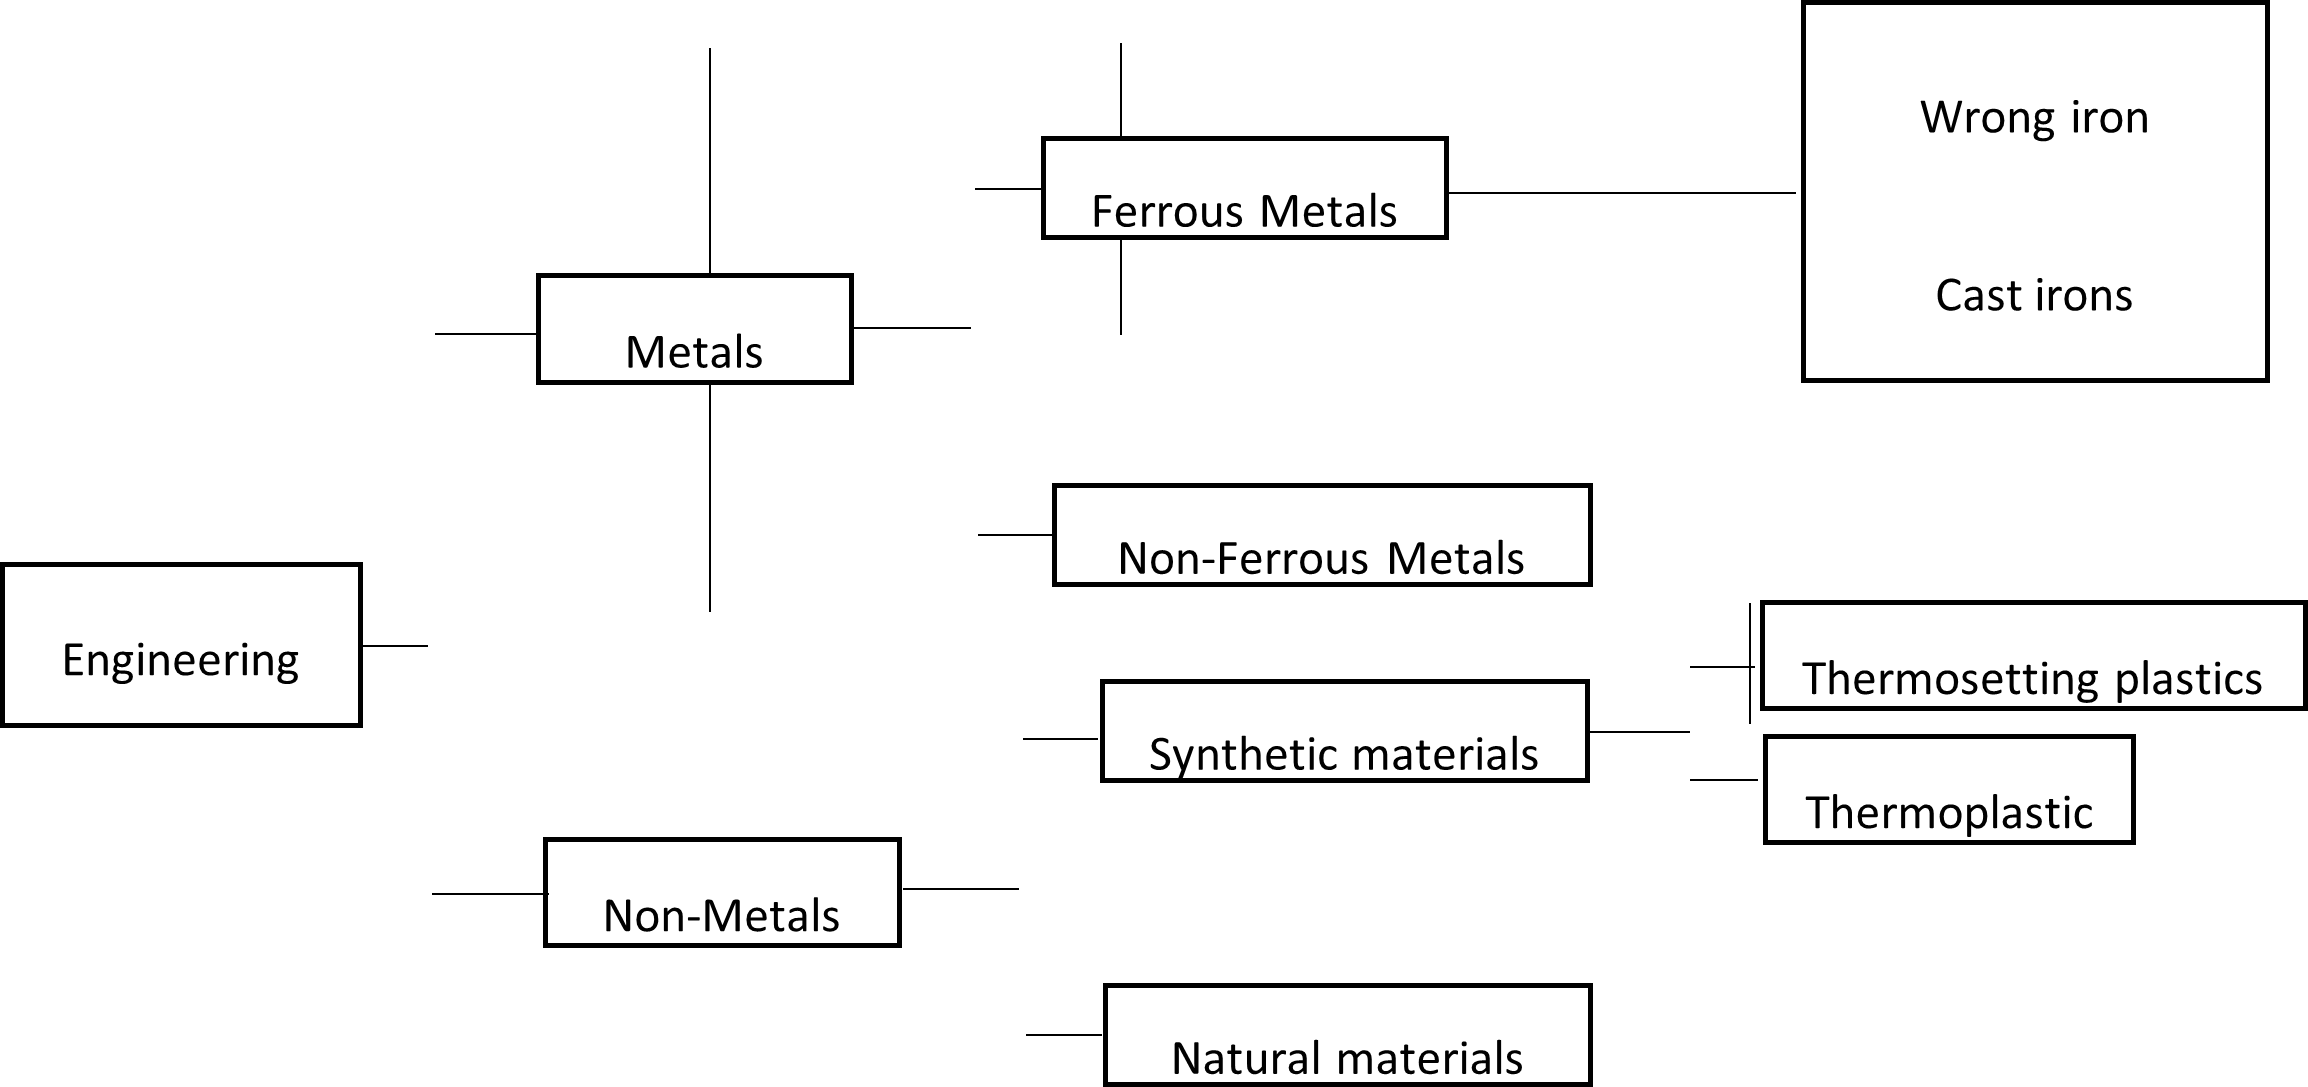
\includegraphics[width=\textwidth]{materials_classification.png}
    \caption{Engineerin materials classifaction [27]}
    \label{ch3:figure:materials}
\end{figure}

Material selection is not a new era, it is a large and traditional branch of engineering materials. Moreover, it requires technical expertise. Material properties can be decisive when evaluating the storage facility material of construction. Material property is defined as an intensive property of a material that is not influenced by the amount of the material [28]. Typically, these are the properties we can measure or test. These properties can continuously interfere with the product stored in the storage tank; hence it is crucial to thoroughly comprehend them. There are several properties of materials, but in the present study, the following broadly properties: physical and mechanical will be carefully investigated, with an effort of improving these properties, thus ensuring the compatibility of the storage facility material of construction with AFFF concentrate.
It is vital to decide whether you are investigating the properties of the material or an object, as this could cause the contradiction. For example, you should decide whether you are identifying the properties of the storage facility or the properties of the material it is constructed of. Properties such as shape and mass of the object (storage facility) may vary, even when they are constructed of the same material. It is for the same reason why it is assumed that the construction structure of the storage facility can have an impact on the performance parameters of AFFF.  In other instances, material properties can be improved by processes such as mixing, heating, and cooling (heat treatment). This may be useful as the improved properties may yield better performance. For this reason, it is of great significance to evaluate the surrounding environmental factors that may change the initial material properties, thus affecting the AFFF concentrate in that process.
Traditionally, storage facilities were constructed using metallic materials. However, in the last decade, researchers have developed specialized non-metallic materials in the form of composite materials to enhance materials that are utilized to construct storage facilities. These exceptional materials have diverse and combined properties that produce an even better performance of storage facilities. Nevertheless, these advanced materials have some limitations and challenges that are notable during the specialized manufacturing technique. 
This section gives an overview of the current materials that are used to construct the AFFF concentrate storage facilities. First, the material characteristics and properties of metallic materials are discussed and carefully evaluated. Since non-metallic materials are gradually emerging, then their properties and limitations are also discussed. Finally, the four common materials used in the present study are specified, and various concerns regarding these materials are analyzed to identify and close the possible gaps that currently exist.   

\subsection{Metallic materials}
Metallic materials are a significant part of engineering materials and have been extensively studied and used for a variety of purposes.  In material sciences, metallic materials are inorganic substances that usually contain a combination of metallic elements, which may also contain small amounts of non-metallic elements [29]. The typical combination of metallic elements could be metals such as gold, iron, titanium, and aluminum, etc. The small amount of non-metallic could be elements such as carbon, nitrogen, and oxygen, etc [25]. In physical sciences, there are 118 elements on the periodic Table, and 86 of these belong to the metallic group [29]. All these 86 metals have diverse characteristics, and a limited number of these can be significantly used for engineering and other purposes.  
In the last century, scientists have been working tirelessly to significantly understand these types of materials to develop efficient techniques that will aid in the optimization of metallic materials. With that being said, over the last 70 years, scientists have developed new techniques for producing various materials with enhanced properties to those of natural materials [29]. To date, numerous metallic materials such as gold and copper mostly rely on these new techniques to yield effective performance. Consequently, metallic materials are rarely utilized as authentic elements, thus they are usually blended with other elements to form an alloy [25]. Many storage facilities are constructed using alloy metals due to their distinctive characteristic properties.
The metallic materials are broadly classified as ‘ferrous and non-ferrous’ [29]. Ferrous metals are those that contain iron (Fe) element within them, while non-ferrous metals do not contain any iron element. In the present study, only ferrous metals will be discussed. Ferrous metals are vital in the present study, as mild and stainless steel materials will be experimentally evaluated when used as AFFF storage facility.  Mild and stainless steels are regarded as ferrous metals due to the presence of iron in their structure. Usually, ferrous metals suffer from the ‘corrosion phenomenon’ due to the presence of iron. The ferrous materials constitute more than 50\% of the metallic materials section [29]. Furthermore, these materials (ferrous) are useful in numerous applications as they meet the various service requirements of our modern and complex society.
While scientists have managed to develop efficient techniques for producing metals, it was of great importance to understand the relationship of structural elements of the materials and their properties. In the textbook ‘engineering materials science’ by Mcarthur and Spalding [28], the microstructure is defined as the arrangement of crystals (or grains) of the different phases. Hence, these are observed when a polished section through a piece of the material is viewed at high magnification through a microscope[30].The chapter of metallic materials has been studied extensively. As a consequence, it has been experimentally proven over the past decades that properties of metallic materials are interrelated with the microstructure of the material itself. This is evidence that the properties can be enhanced by altering relative proportions of the micro-constituents (or phases). Phases are identified by their unique crystal structures, composition, and properties [28].
Liquid storage facilities are critical in ensuring that the properties of the stored products are well maintained. Metallic materials have offered numerous and diverse benefits when utilized as liquid storage facilities. However, in other instances horrible incidences that result in storage facility catastrophic failure occur. This proves that although metallic materials are beneficial, there are still gaps that exist, probably in the metal production optimization, enhancing of natural properties, and relevant materials selection. There are relatively three factors that may influence the choice of metals and alloys when used as AFFF storage facility:

\begin{itemize}
    \item Mechanical, physical, chemical, and thermal properties.
    \item Degradation of the material.
    \item Compatibility with the product to be stored, which is AFFF for the present study.
\end{itemize}

Understanding relevant material selection will aid in easing the enhancement of the properties of metallic materials. This will be more useful in metallic materials that are widely utilized to construct the storage facility for storing AFFF concentrate. 

\subsection{Metalic bonding}
In general, the term ‘bonding’ can be described as the action of joining two or more things firmly, especially employing adhesive, heat, or chemical bonds [31]. In materials and science, there are three (3) types of bonding: covalent, ionic, and metallic bonding. For the present study, the focus will be on evaluating and comprehending metallic bonding.
In the early 1900s, Paul Drüde discovered the metallic bonding theory by modeling metals as a mixture of atomic cores (positive nuclei + inner shell of electrons) and valence electrons [32]. The metallic bonding can be described as the type of chemical bond formed between positively charged atoms in which the free electrons are shared among a lattice of cations [33]. In contrast, covalent and ionic bonds form between two distinct atoms. Metallic bonding in the major type of chemical bonding that forms between metal atoms. Figure \ref{ch3:figure:bonding} shows how a metallic bond occurs.

\begin{figure}[H]
    \centering
    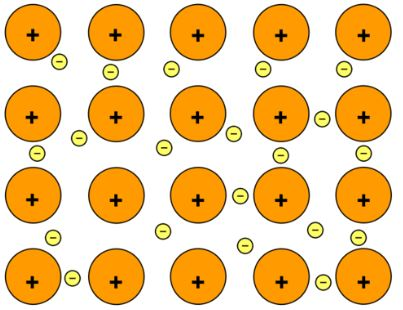
\includegraphics[width=.5\textwidth]{metalic_bonding.jpg}
    \caption{Metalic bonding: Positive atomic nuclei (orange circles) surrounded by delocalized electrons (yellow cirlces)[31].}
    \label{ch3:figure:bonding}
\end{figure}


Metallic bonds are commonly noticed in natural metals, alloy metals, and some metalloids. For instance, graphene (an allotrope of carbon) usually reveals two-dimensional metallic bonding [33]. It should be noted that metals, including the natural ones, are not limited to metallic bonding. Thus, they have the capability of forming other types of chemical bonds within their atoms.
All atoms contain a small nucleus of neutrons and protons these are surrounded by the orbiting electrons [25]. Distinct atomic models can be significantly used to describe different properties of the overall material. As previously stated, one beneficial model of a metal is a repeating structure metallic ion, which are surrounded by a ‘sea’ of electrons, see Figure \ref{ch3:figure:bonding}. It is the ‘free electrons’ that critically determines the thermal and physical properties of the metallic material [25]. Alternatively, several mechanical properties of metallic materials can be better understood by considering atoms to behave like ‘hard spheres’ [25]. This is vital in the present study as this will be used as a benchmark in improving the properties of alloy metals that are commonly utilized as AFFF storage facility.
When atoms are behaving like hard spheres, they are relatively bonded together by an attractive force [33]. However, this type of bonding is very weak, which is the reason why metals have a crystalline structure where atoms are significantly arranged in a dense, regular, and repeating manner. The atoms of various metals are significantly arranged in various crystal structures [25]. Atoms in metallic materials can be relatively arranged in four (4) different ways these include face-centered cubic (f.c.c), hexagonal closed pack (h.c.p), body-centered cubic (b.c.c) and tetragonal. A typical example may include a pure metal such as aluminum (Al) in which atoms are relatively arranged in f.c.c at room temperature [25], as shown in Figure \ref{ch3:figure:aluminium}.
 
\begin{figure}[H]
    \centering
    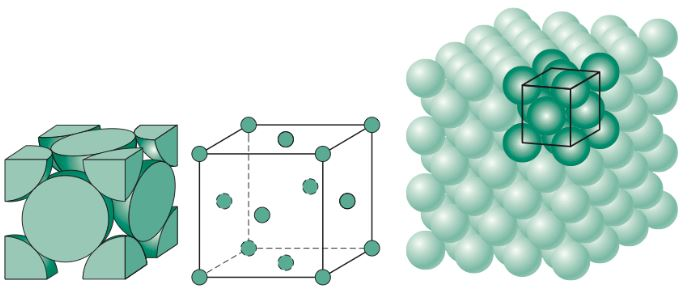
\includegraphics[width=\textwidth]{aluminium_crystal_structure.jpg}
    \caption{Crystal structure of aluminium metal (Al) at room temperature [25].}
    \label{ch3:figure:aluminium}
\end{figure}

The mentioned crystal structures are determined at room temperature.  However, the transition in the crystal structure is much possible in several metals. This transition varies with the temperature in which the metal is exposed to [34]. For example, metals such as pure iron may reveal two (2) different crystal structures. At room temperature it reveals b.c.c, but when the temperature is constantly increased towards a melting point (912-1394℃), its crystal structure changes to f.c.c. Further increasing the temperature to about 1538 ℃ will result in reverting the crystal structure to b.c.c [29, 30].For alloy metals, the transition in the crystal structure can be achieved by adding an element with a different crystal structure. The transition in alloy metals will be evaluated in detail in section 3.6. Table \ref{ch3:table:structure} shows the atom arrangement in a crystal structure of some commonly used pure metals.

\begin{table}[H]
\caption{Crystal structure for popular metals, at room temperature [25].}

\centering
\begin{tabular}{ c c c }
    \hline
    Metal & Crystal structure \\
    \hline
    Aluminum & FCC \\
    Chromium & BCC \\
    Copper & FCC \\
    Gold & FCC \\
    Iron & BCC \\
    Silver & FCC \\
    Nickel & FCC \\
    \hline
\end{tabular}

\label{ch3:table:structure}
\end{table}

Several physical and mechanical properties of materials are determined by the metallic bonds and the arrangement of the atoms in the crystal structure. For example, when metallic material is heated to a melting point, the atoms have to gain sufficient energy to break free from the crystal structure [25]. This is evidence that the properties of materials can be altered by altering the arrangement of atoms in a crystal structure. Moreover, the crystal structure significantly determines the ability of atoms to slip over one another during the deformation of metals [34]. This is especially true in ductile metals due to their ability to deform without easily breaking. These types of materials are commonly used to construct liquid storage facilities due to their crystal structure that yields exceptional properties.

\section{Mild steel the material}
Mild steel is a ferrous metal that contains a relatively low content of carbon, which usually ranges from 0.05\% to 0.25\% by weight [34]. Thus, it is also known as 'low-carbon steel.  Low carbon steels consists primarily of ferrite rather than perlite [35]. Metals containing carbon content from 0.30 to 2.0\% are typically referred to as higher carbon steel [27]. The addition of carbon content increases the strength of the steel. Consequently, steel materials having a carbon content higher than 2\% are often regarded as ‘cast-iron' [34].  Mild steel is a popular metallic material that has been extensively used for many applications, including industrial storage facilities.
Although mild steel contains carbon, iron, and other elements in its composition, it nonetheless cannot be regarded as alloy steel. This is due to the extremely low amount of carbon and other alloying elements it contains; thus, these elements are insufficient to produce alloy steel. The relatively low amount of carbon and other alloying elements in the composition of mild steel results in diverse properties when compared to higher carbon and alloy steels [27]. The high content of iron and ferrite in the composition of mild steel means that it is magnetic [35].
Low-carbon steels are generally useful in liquid storage facility construction, due to their compatible properties. In particular, mild steel is one of the most commonly used tank construction materials. It is popularly known for its ductility and can be made from readily available natural materials. The low cost of this metal makes it beneficial to numerous industries in terms of economic.
The low-carbon steels set back up to date is the degradation due to corrosion, which causes more serious deterioration problems to storage facilities[36]. Various coatings have been developed over the past decade years, aiming to mitigate this problem. The other major concern regarding low-carbon steels is that it is nearly impossible to alter some of the mechanical properties through heat treatment [34]. Moreover, low-carbon content means that mild steel has very little alloying elements to prevent the dislocation in the crystal structure, thus resulting in less tensile strength than high carbon and alloy steels [34].
This section provides and evaluates mild steel as a material and also as an object (storage facility). The scope of this section includes the evaluation of the current properties and their impacts on the AFFF storage facility. Similarly, the understanding of the microstructure of low-carbon steels to develop useful strategies to improve the properties and compatibility of this metallic material is essential for the present study. The machinability of low-carbon steels is evaluated. Furthermore, the corrosion concerns are discussed, and common methods to prevent this are briefly discussed. Finally, the heat treatment processes that are commonly used to enhance the properties are also closely assessed. This will aid in understanding the gaps in the optimization of the properties

\subsection{Useful properties} 
As previously stated, the material property is a comprehensive property that is not dependent upon the amount or size of the material [37]. These are the quantitative parameters that are measurable/tested and observed when a load is applied. As a consequence, these properties are significantly determined by the composition and crystal structure of the material. Thus, it is vital to understand the arrangement of atoms in the crystal structure. Furthermore, before any material is selected for a certain application, the properties should be immensely understood to ensure the compatibility with the application utilized.
Mild steel has a variety of properties that makes it beneficial for several applications and these are detailed in Table B.2 on appendices. These properties can be broadly grouped into mechanical and physical properties [37]. These two properties are a vital determinant for which metal is considered to be compatible with a given application. In almost every instance, mechanical properties are interdependent, meaning high performance in one category may be achieved with lowering performance in other categories [37]. For example, low content of carbon in mild steel means that this metallic material is more ductile when compared to alloy steels. 
For low carbon steels, ductility indicates that they can be formed into the desired shape in any temperatures without major difficulties [38]. Figure \ref{ch3:figure:carbon} shows how the carbon content of plain carbon steel affects the properties of the steel. Referring to Figure \ref{ch3:figure:carbon} it can be observed that altering carbon content in plain carbon steels has an impact on the properties. Consequently, when the carbon content has increased, the ductility of the steel materials is relatively decreased. Moreover, the strength and hardness are remarkable increased, which results in the transition from ductile to brittle [39]. For liquid (AFFF) storage facilities, ductility is one of the significant properties. This property means that the storage facility can be rolled or joined using various mechanical fabrication methods mentioned in section 4.3.1, without having major concerns.
 
\begin{figure}[H]
    \centering
    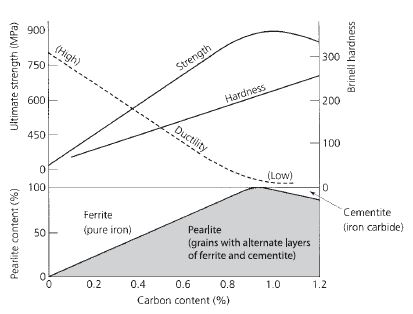
\includegraphics[width=.65\textwidth]{effect_of_carbon_content.jpg}
    \caption{Effect of carbon content on the properties of plain carbon steel [27].}
    \label{ch3:figure:carbon}
\end{figure}

Another critical parameter for storage facilities constructed of mild steel is thermal conductivity, which falls under physical properties. In the textbook, ‘heat transfer: a practical approach’ by Cengel [40] thermal conductivity is defined as a measure of the quantity of heat that flows through a material. In the present study, the storage facility does not necessarily need to be constructed with materials that have a high thermal conductivity. However, achieving this is somehow difficult, due to diverse properties a material can have.
Mild steel has a thermal conductivity of 64.86 $\nicefrac{W}{m.K}$ at most [40]. This is quite less when compared to other steels but can be considered high for applications that do not require heat transfer. At extremely high temperatures, heat may be transferred to the product inside the storage tank and may influence the viscosity of the product. For the present study, heat transfer is not a concern, due to the environment (atmospheric), the storage facility is located on. However, when looking at this from another perspective, it can cause problems along the time. When the storage facility is continuously exposed to high-temperature environments, heat can be gradually transferred until it causes some notable problems to AFFF solution. To reduce heat transfer, insulating materials are usually utilized, but they however do not eliminate the problem completely. As a consequence, it is vital to understand the environmental factors that may associate with the properties of the material on the location of the storage facility.
There are normally three means of transferring heat namely conduction, convention, and radiation. Conduction involves heat transfer through solid materials, convention is associated with heat transfer between a solid surface and a gas or liquid that is in motion, while radiation is the energy emitted by the matter in the form of electromagnetic waves [40]. In case of AFFF storage facilities, heat transfer by conduction is of great interest, as this is the possible scenario on this circumstance.   
For the worst situation, the total heat energy that can be transferred to the storage facility, hence AFFF concentrate as a result of the surround atmosphere (radiation) can be calculated using energy balance equation as follows:

\begin{equation}
    Q_c = m \times C_p \times \Delta T
\end{equation}

\noindent Where, \\
$Q_c\ is\ the\ amount\ of\ net\ heat\ transfer\ to\ the\ system\ in\ J$ \\
$m\ is\ the\ mass\ of\ amaterial\ in\ kg$ \\
$C_p\ is\ the\ specific\ heat\ capacity\ in\ \nicefrac{kJ}{kg.^\circ C}$ \\
$\Delta T\ is\ the\ temperature\ difference\ of\ surfaces\ in\ ^\circ C$ \\

When the total heat energy that is being transferred to the storage tank holding AFFF is known, it is now vital to estimate the rate at which this heat energy is being transferred. This is critical in predicting whether the composition of AFFF concentrate are being affected by the heat that is transferred to the storage facility by conduction. The equation for calculation of conduction heat transfer rate is known as Fourier’s Law of Heat Conduction and is given by:

\begin{equation}
    Q_c = -k \times A \times \frac{\Delta T}{\Delta r}
\end{equation}

\noindent Where, \\
$Q_c\ is\ the\ conductive\ heat\ transfer\ rate\ in\ W$ \\
$k\ is\ the\ thermal\ conductivity\ of\ thematerial\ in\ \nicefrac{W}{m.^\circ C}$ \\
$A\ is\ the\ cross-sectional\ area\ in\ m^2$ \\
$\Delta T\ is\ the\ temperature\ diifference\ of\ surfaces\ in\ ^\circ C$ \\
$\Delta r\ is\ the\ distance\ separating\ the\ surfaces\ in\ m$ \\

In heat transfer, positive heat conduction means that heat is flowing into the body in question, and negative heat conduction represents heat leaving the body. Heat transfer has been applied in various research fields mainly to increase the heat transfer rate, decrease heat transfer rate and keep the temperature in a certain range. For the present study the focus is to ensure the decrease in the rate of heat transfer, so that it will not suddenly change the composition of AFFF, thus influencing its firefighting performance.  
Another property of interest for the present study is the effect of corrosion on steels. Corrosion is the process of decay of a material (usually ferrous metals) caused by chemical reaction with its environment [41]. AFFF concentrate is generally not a corrosive type of liquid. However, mild steel contains about 98\% of iron on its composition, which is significantly high and makes it to be considered as a corrosive ferrous metal.  The corrosion phenomenon is usually prevented in several ways, and these will be discussed in detail in section 3.5.

\section{Stainless steel the material} 
Stainless steels are ferrous metallic materials that contain a minimum of 10.5\% of chromium and about 8\% of nickel as main alloying elements [42]. All the alloying elements have a significant role in the stainless steel family. Chromium element forms a protective self-healing oxide film, which greatly improves the corrosion resistance of stainless steel [30]. Large amounts of nickel contribute to both heat and corrosion resistance [43]. However, depending on the percentage of nickel added, it also contributes to high strength and excellent toughness. Other relevant elements are often added to enhance the properties of stainless steel. It is these alloying elements that make stainless steel to be generally more expensive than carbon steels.
The classification of stainless steel is based on the nature of their metallurgical structure [44]. As previously stated in 3.2, the metallurgical structure is the arrangement of the atoms making up the grains of the steel. The microstructure is formed based on the chemical composition of the steel. With an appropriate combination of alloying elements that results in a unique microstructure, stainless steels can be fully austenitic, a mixture of ferrite and austenite (duplex), fully ferritic or martensitic [44]. These four possible microstructure phases are shown in Figure \ref{ch3:figure:steel_phase}. These categories of stainless steel are obtained under specific cooling conditions, and all are beneficial for various applications.
 
\begin{figure}[H]
    \centering
    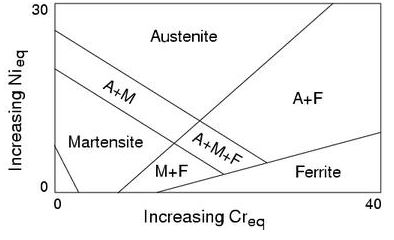
\includegraphics[width=.65\textwidth]{stainless_steel_phase.jpg}
    \caption{Stainless steel phase diagram as a function of chromium and nickel equivalents at room temperature [44].}
    \label{ch3:figure:steel_phase}
\end{figure}

In the present research work, duplex stainless steel is of great significance. As can be seen in Figure \ref{ch3:figure:steel_phase}, duplex contains a combination of austenite and ferrite, approximately 50\% of each. It is more beneficial and extensively used in liquid storage facilities, as it yields in a combination of properties. This is due to a large amount of chromium and less nickel content presence, which results in corrosion resistance, high strength, and excellent toughness [45]. The weighed composition of duplex stainless steel is detailed in Table B.3 on appendices. The less content of nickel in duplex stainless steel implies that duplex is relatively inexpensive compared to other classes [42]. The two-phase mixture also reduces the risk of intergranular attack; for the same reason, they are not prone to solidification cracking during welding [42]. Figure \ref{ch3:figure:weight} shows the comparison of the weight percentage of chromium (Cr), nickel (Ni), and molybdenum (Mo) in duplex and austenitic stainless steel.
 
\begin{figure}[H]
    \centering
    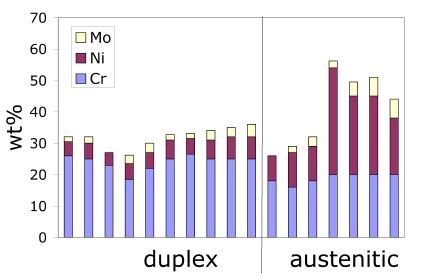
\includegraphics[width=.65\textwidth]{weight_percentages.jpg}
    \caption{Weight percentage of Cr, Ni, and Mo in duplex and austenitic steels [42].}
    \label{ch3:figure:weight}
\end{figure}

In general, stainless steel is an excellent metallic material that has several useful properties which are shown in Table B.4 on appendices. Consequently, this type of steel offers numerous benefits for various applications. Although stainless steel is popularly known for excellent corrosion resistance, reports in recent years have suggested otherwise [46]. Corrosion in stainless steel often occurs unexpectedly on the welded joints, which then affects the product that is stored, particularly in welded storage tanks applications. Another concern for stainless steel is the difficulty in machinability [47]. Fabricating or manufacturing stainless steel is not an easy task, due to the elements it contains. All these concerns are greatly dependent on the microstructure of the material, and the possible optimization methods will be discussed in sections 3.6 and 3.8 respectively.

\section{Effect of corrosion on steels}
Corrosion is an integrative and critical subject of matter that has numerous half-truths and myths, which exist to date [28]. These are continuously occurring due to ignorance when it comes to the science of corrosion.  Corrosion is the phenomenon that commonly affects ferrous metals due to the presence of iron. In corrosion science, corrosion is defined as the deterioration of a substance or its properties due to interactions between the substance and its environment [48].
In recent years, corrosion has become a vital matter in liquid storage facilities, especially in acidic liquids. Corrosivity is generally measured by either pH or the rate of steel corrosion [49]. When the aqueous solution has a Ph less than or equal to 2, or more than or equal to 12.5, it is considered to be corrosive [49]. As a consequence, corrosion is generally not a concern on storage facilities containing AFFF concentrate since it has an approximate Ph value of 7-8.5. However, the storage facility can nonetheless suffer from corrosion due to the surrounding environment. In the present research, a storage facility containing AFFF concentrate is continuously exposed to the corrosive atmospheric environment (Durban, South Africa) due to the near sea. Figure \ref{ch3:figure:ph} shows the corrosive Ph level of an aqueous solution. 
 
\begin{figure}[H]
    \centering
    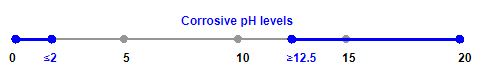
\includegraphics[width=.8\textwidth]{aqueous_solution_ph_scale.jpg}
    \caption{Ph scale for aqueous solution [49].}
    \label{ch3:figure:ph}
\end{figure}

Although there is a lack or little knowledge of the corrosion phenomenon, some researchers have made significant efforts to understand it. The material is initially selected due to the desired properties. However, some recently published literature suggest that corrosion has a degrading effect on mechanical properties. Mahmoodian et al [35] conducted a study that concluded that corrosion can lead to a reduction of the thickness of the storage facilities, and thus in the reduction of yield strength, ultimate strength, and ductility on low carbon steels.  Marcus [50] further stated that the reduction of these properties is due to hydrogen accumulation within the steel, which is known as hydrogen embrittlement [HE). Besides, this accumulation of hydrogen results in a sudden reduction in the ductility of steel. Figure \ref{ch3:figure:degradation} shows the process of mechanical properties degradation due to corrosion.
 
\begin{figure}[H]
    \centering
    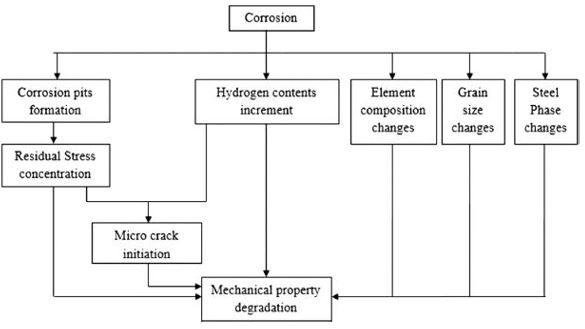
\includegraphics[width=\textwidth]{process_of_mechanical_properties.jpg}
    \caption{Process of mechanical properties degradation due to corrosion [50].}
    \label{ch3:figure:degradation}
\end{figure}

In more detail, corrosion occurs when there is a combination of oxygen reduction and hydrogen evolution reactions, as shown in equations \ref{ch3:equation:acid} – \ref{ch3:equation:neutralalkaline} [35].  Consequently, during these reactions, atomic hydrogen is released. It then eventually accumulates at the defects within the steel, forming molecular hydrogen. Finally, the molecular hydrogen results in the increase of inside pressure, and eventually micro-cracking initiations, which consequently degrades the mechanical properties of steel [51].

\begin{center}
    Oxygen Reduction Reaction (ORR)
\end{center}

\begin{equation}
    \frac{1}{2}0_2 + 2H_3O^{+2e \rightarrow 3H_2OAcid}
    \label{ch3:equation:acid}
\end{equation}

\begin{equation}
    \frac{1}{2}O_2 + H_2O + 2e \rightarrow 2OH^{-Neutralalkaline}
\end{equation}

\begin{center}
    Hydrogen Evolution Reaction (HER)
\end{center}

\begin{equation}
    H_3O^{++e \rightarrow \frac{1}{2}H_2 + H_2OAcid}
\end{equation}

\begin{equation}
    H_2O + e \rightarrow \frac{1}{2}H_2 + OH^{-Neutral,alkaline}
    \label{ch3:equation:neutralalkaline}
\end{equation}

Based on equations \ref{ch3:equation:neutralalkaline} – 3.9, it is sensible to believe that corrosion changes the elemental composition of the steel. However, few papers focus on monitoring the changes in element composition during corrosion. Corrosion may also result in the degradation of mechanical properties by changing three microstructural features: (1) grain size, (2) phase composition, and (3) formation of corrosion pits [35]. Presumably, corrosion is interrelated with the microstructure of the material. For example, grain size reduction causes more hydrogen absorption within steel [35]. However, there are several limitations to existing Research. To begin with, the hydrogen embrittlement phenomenon has been mainly carried out for high-strength low-alloy steel (HSLA) and stainless steel [35]. As a consequence, extensive research should be conducted to determine the degradation mechanism of mechanical properties due to corrosion, at both macro and micro levels.  
Many researchers have been interested in the corrosion phenomenon, thus over the years, there have been several ways developed to prevent corrosion. Corrosion can occur in many ways, thus it also significant to understand different types of corrosion and evaluate the corrosion of interest. Stainless and mild steel are the metallic materials of interest in the present study; thus, it is vital to understand the different ways in which corrosion occurs in these two metallic materials. In this way, it is possible to optimize the current methods that are utilized to prevent corrosion, focusing precisely on the corrosion of interest.
As previously stated, several half-truths and myths regarding corrosion exist. Stainless steel is popularly known for resisting corrosion due to the presence of a chromium element in its composition. However, these are myths and half-truths due to the incidences that have proven that stainless steel can suffer from corrosion. This is usually the case on welded products. In contrast, mild steel is well known for suffering from corrosion, this is due to the lack of corrosion protecting alloying elements such as chromium [52]. However, corrosion prevention is more practical than making an effort to eliminate it completely. A stainless steel storage facility that has suffered from corrosion on welded joints is shown in Figure \ref{ch3:figure:tank}.
 
\begin{figure}[H]
    \centering
    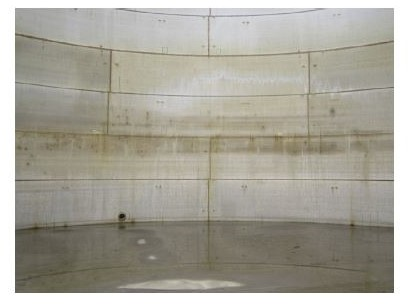
\includegraphics[width=.55\textwidth]{storage_tank.jpg}
    \caption{Storage tank that corroded on welded joints [46].}
    \label{ch3:figure:tank}
\end{figure}

\subsection{Types of corrosion} 
The tendency of a metal to corrode depends upon the crystal structure of the metal, its composition as formed during alloying, and the temperature for deformation of a single metal surface developed during fabrication [42]. The environment plays a key role in corrosion of the material; thus, it can vary with the environment in which the substance is exposed. Consequently, this makes it complex to comprehend the corrosion mechanism. Corrosion can be caused by diverse factors that include reactivity of metal, presence of impurities, presence of air, moisture, gases like sulphur dioxide, and carbon [42]. Therefore, corrosion protection and prevention are significantly aimed at addressing these factors. There are various types of corrosion, and it is vital to understand which corrosion you are faced with. The different types of corrosion which depend upon the environment surrounding the material, type of material, or chemical reaction are briefly described in Table \ref{ch3:table:corrosions}.

\begin{table}[H]
\caption{Types of corrosion [48].}

\centering
\begin{tabular}{m{.35\textwidth} m{.65\textwidth}}
    \hline
    Type of corrosion & Description \\
    \hline
    Uniform corrosion & Deteriorates the whole surface of the metal and makes the surface thin. \\
    Galvanic corrosion & Occurs with an electrolyte with metal having different values of electrical potentials. \\
    Pitting corrosion & Occurs because of the random attacks on particular parts of the metal’s surface to form pits. The pit acts as an anode, while the undamaged part of the metal is the cathode. \\
    Stress corrosion cracking & A complex form of corrosion which arises due to stress and  corrosive environment. \\
    Corrosion fatigue & A combination of cyclic stress and corrosion.  \\
    Intergranular corrosion & Corrosion occurs on or near the grain boundaries of a metal.  \\
    Crevice corrosion & Concentration cell corrosion due to the trapping of corrosive liquid  between the gaps of the metal. \\
    Filiform corrosion & Concentration cell corrosion on metallic surfaces coated with a thin  organic film. \\
    Erosion corrosion & Flow-assisted corrosion which is due to the movement of corrosive  liquids on metal surface. \\
    Fretting corrosion & A form of corrosion which shows the combined effect of corrosion and  fretting of metal. \\
    \hline
\end{tabular}

\label{ch3:table:corrosions}
\end{table}

In the present study, the focus is on stress corrosion cracking/atmospheric corrosion. As can be observed in Table \ref{ch3:table:corrosions}, stress corrosion cracking is a complex form of corrosion which arises due to the stress and corrosive atmosphere. However, the cracking of the storage facility due to stresses is not a concern in the present study, thus the focus is particularly on the corrosive atmospheric environment.

\subsubsection{Atmospheric corrosion}
Atmospheric corrosion is a naturally occurring chemical deterioration of a material due to reaction with the environment, and especially with oxygen. The extent of deterioration of a ferrous metal depends on the chemical composition and grain structure of the material. For example, when the iron is exposed to an industrial atmosphere for a long period, iron oxide, also known as rust, forms on the surface, as shown in Figure \ref{ch3:figure:corrosion} [28]. The rust is very porous to oxygen and water in the atmosphere, and consequently, the corrosion process continues until the metal is entirely consumed [50].  The atmospheric corrosion generally occurs in three various environments rural, industrial, and marine. For the present study, the industrial environment is the benchmark since the storage facility is located in an industrial environment. Figure \ref{ch3:figure:corroded} shows the storage facility, which was initially protected from the corrosion yet ended up suffering from rural atmospheric corrosion.

\begin{figure}[H]
    \centering
    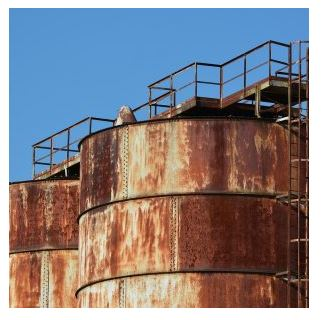
\includegraphics[width=.4\textwidth]{corrosion_of_storage_facilities.jpg}
    \caption{Atmospheric corrosion of storage facilities in industrial environment [48].}
    \label{ch3:figure:corrosion}
\end{figure}
 
\begin{figure}[H]
    \centering
    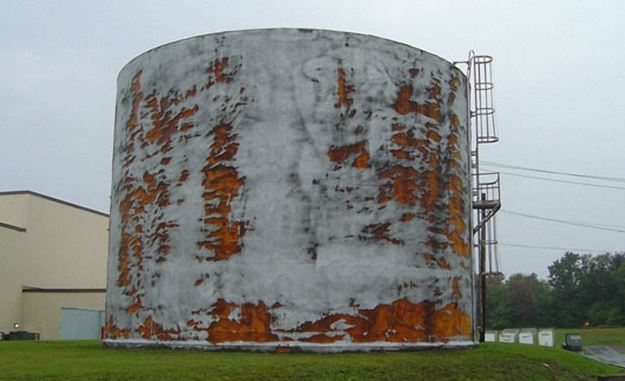
\includegraphics[width=\textwidth]{corroded_storage.jpg}
    \caption{Corroded storage facility [50].}
    \label{ch3:figure:corroded}
\end{figure}

Atmospheric corrosion is one of the most common types of corrosion, which is affected by several environmental factors. It commonly affects infrastructure, transportation, energy, and other industries [53]. Over the decades, the research has shown that contributing environmental factors affecting the outdoors atmospheric corrosion rate include: temperature, relative humidity (RH), atmospheric pollutants (commonly sulphur dioxide and chlorides), and wind [39, 41]. It is difficult to individually analyse the impact of these factors due to the existence of complex interaction between them.
In the past years, several researchers have made significant efforts in analysing the influence of the single factor on atmospheric corrosion. Cai et al [54] studied the effects of RH, temperature, sulfur dioxide, and chlorides on the short-term corrosion behaviour in the dynamic environment. They demonstrated that RH is the most influential factor in corrosion, and the temperature is secondary. The effect of RH can be reflected by the time of wetness (TOW) according to ISO9223 by the International Standardization Organization (ISO) [40, 41]. In 2020, Pei et al [53] further investigated the environmental impacts of RH, temperature, and rainfall on the initial corrosion behaviour of steels. The outcomes showed that rainfall is the most influencing factor in the initial atmospheric corrosion rate.  Moreover, RH significantly influenced the corrosion of steels in low precipitation environments and non-rainfall period.
The environmental conditions are natural; thus, they keep changing unexpectedly. With this regard, it becomes difficult to predict the effect of a dynamic environment on atmospheric corrosion. Nevertheless, a model that predicts the corrosion loss as a function of environmental parameters and exposure time is required. Cai et al [54] suggested that to develop the model that will be effective in a dynamic environment, firstly, a corrosion kinetic model is required to predict the corrosion process over time. Then, a parametric method is necessary to describe the precise dynamic environmental factors. And finally, an accelerating model that describes the effects of environmental factors on the corrosion rate is essential to correlate the corrosion parameters with the environmental factors [55]. All these conditions exclude the effect of rainfall. The effect of acidic rain of the corrosion effect is very complex, thus is not understood fully [53]. However, the use of corrosion (and environmental) monitoring techniques is highly desirable.

\paragraph{Effects of atmospheric factors on corrosion} 
Over the past years, researchers have successfully demonstrated that the atmospheric corrosion effect of environment on the metals comprises of three (3) main components parts: the effect of dry deposition of sulphur dioxide, the effect of dry deposition of chloride, and the effect of wet deposition of hydrogen ions (acid rain) [54].
The amount of rainfall and acidity of the precipitation can be measured using a couple of existing exposure programs such as The Ibero-American Map of Atmospheric Corrosiveness (MICAT) project, the On-site Stormwater Detention (OSD) program, and the United Nations Economic Commission for Europe (UN/ECE) program [54]. However, the existing data are limited, thus the quantitative models or programs cannot be successfully developed. Moreover, the lack of experimental data on the impact of hydrogen ions on atmospheric corrosion rate means that it is excluded from ISO 9223 [50]. The factors affecting the atmospheric corrosion are listed below.

\begin{itemize}
    \item \textbf{Relative humidity:} As stated previously, RH has a greater influence on the atmospheric corrosion of steels. The relationship between atmospheric corrosion rate and RH has been demonstrated by several researchers [38, 41]. In addition, according to many researchers and scientists, the corrosion rate is directly proportional to RH [38, 41].Technically, when RH is increased in an environment the rate of atmospheric corrosion is also increased. RH is, however, independent of any other atmospheric factor. For example, when RH is increased typically from 75\% to 95\%, the rate of corrosion will increase regardless of the temperature [42]
    
    \item \textbf{Temperature:}  Researchers have demonstrated that temperature also has a huge impact (behind RH) on atmospheric corrosion [41, 40]. However, the relationship of temperature on atmospheric corrosion is complex, and thus can be represented in two aspects: the direct influence on corrosion reaction rate and influence on electrolyte film formation [54]. To predict the effect of temperature, the corrosion rate is correlated with ambient temperature [53].  This is achieved by Arrhenius law, which is based on Can't Hoff’s equation [54]. Based on the Arrhenius equation, it has been mathematically proven that corrosion rates will increase by up to 15\% if temperature increases by 2 ℃ [28]. However, more studies are required to quantify the effect of temperature on atmospheric corrosion rate.  
    
    \item \textbf{Environmental pollutants (Sulphur dioxide and Chlorides):} Atmospheric corrosion rate can also be increased by the chemicals that have ended up in the environment due to activities of human and sometimes negligence. These types of chemicals are usually dangerous or hazardous to human health. In many works, it is found that environmental pollutants are proportional to the rate of atmospheric corrosion [31, 38, 41]. For example, Cai et al [54] indicated that sulphur dioxide will be oxidized to sulfate ion (SO4-2) in the water, which produces the hydrogen ions (H+) and thus increases the acidity of electrolytes. In this way, the corrosion rate is significantly increased, which results in the dissolution of the corrosion product.
\end{itemize}
    
On the other hand, the deposition of chlorides results in the acceleration of atmospheric corrosion, especially for steels [41]. When chlorides deposit on the metal surface, the electrolyte conductivity increases as well as the TOW of the metal surface, which then rapidly increases the rate of atmospheric corrosion on steel materials [49]. However, chloride is commonly influenced by rainfall and surface temperature [54].

\section{Microstructure morphology} 
It was discussed previously in section 3.2, that many properties of steels depend upon the microstructure and the atomic bonding. The fundamentals of microstructures of steel and iron should be closely related to the iron-equilibrium diagram. The iron-carbon diagram significantly provides valuable details regarding the behaviour of both plain carbon and alloy steels in their immense variety [44]. 
Microstructures of steels critically determine the mechanical, physical, and chemical properties of a material. For example, the strength and hardness of materials are critically determined by the number of phases and their grain sizes [57]. Microstructures cannot be described by a single factor. Thus a complete description of microstructures involves describing the size, shape, and distribution of grains and second-phase particles and their composition; and also the defect structures, although these are often omitted [58]. In simple terms, the microstructure can be described as the very small scale or microscopic structure of a material. These microstructures can be observed using various microscopic techniques.  
The resulting properties of steels are often controlled by several microstructural features. These features include two-dimensional defects such as grain boundaries and heterophase interfaces, one-dimensional defects such as dislocations, and zero-dimensional defects such as point defects [57]. However, the enhancement of the resulting properties is possible through controlling the atomic arrangement and microstructure using various optimization processes such as casting, powder metallurgy, working, and heat treatment. During these optimization methods, steels are subjected to various microstructural phases.

\subsection{Ferrite} 
Iron is a pure metal that can be microscopically thought of as a 3-D lattice of stacked billiard balls. Iron is dominant in most low carbon steels, hence the 99\% of the microstructure is still iron, with all other elements combining to form typically less than 1\% of the overall composition [59]. However, no matter how well billiard balls are packed, they will always be small gaps between them. These small gaps are commonly known as interstices [59]. Nevertheless, the smallest elements like carbon and nitrogen can fit in these gaps, as shown in Figure \ref{ch3:figure:gaps}. As alloying increases, the straining in the atomic lattice increases, requiring more force to deform a work piece, thus increasing the strength. When a very small portion of the interstices in between the iron lattice is occupied by carbon atoms, this interstitial-free (IF) steel is said to have a microstructure of ferrite [44]
 
\begin{figure}[H]
    \centering
    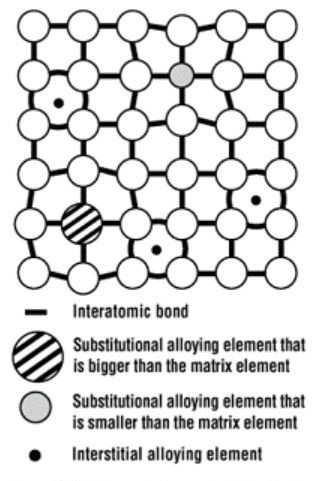
\includegraphics[width=.5\textwidth]{small_gaps_between_atoms.jpg}
    \caption{Small gaps between atoms, called “interstices” [59].}
    \label{ch3:figure:gaps}
\end{figure}

Ferrite is a solid solution of iron, containing carbon, or one or more alloying elements, such as silicon, chromium, manganese, and nickel [30]. In addition, it has an interstitial solid solution and a substitutional solid solution. Since the carbon elements have occupied the interstices, larger elements such as manganese, magnesium, silicon, and phosphorus substitute for iron in the lattice, see Figure \ref{ch3:figure:tank} [60]. However, there is a limitation on how much carbon can occupy the interstices. Commonly, 0.02\% carbon at 725 ℃, but dropping to 0.006\% carbon at room temperature is more than enough to fit in the interstices [44]. Ferrite has a bcc crystal structure with a microstructural phase that is soft, ductile, which is similar to pure iron [59]. The microstructure of ferrite is shown in Figure \ref{ch3:figure:microstructure}.

\begin{figure}[H]
    \centering
    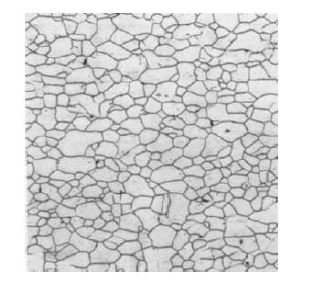
\includegraphics[width=.5\textwidth]{microstructure_of_carbon_steel.jpg}
    \caption{Microstructure of fully ferritic, ultralow carbon steel. Marshalls etch + HF, 300x [30].}
    \label{ch3:figure:microstructure}
\end{figure}

\subsection{Austenite} 
In the phase known as austenite, the interstices are much larger than in the ferrite phase and have the fcc crystal structure, as shown in Figure \ref{ch3:figure:austenite} [59]. This allows more carbon content to occupy the interstices. At critical temperatures, which is around 1,150 ℃, carbon content up to 2\% can fit into the austenite, as the result of larger interstices [44]. As a consequence, in plain-carbon and low alloy steels, austenite phase is not possible to form at room temperature but can only exist in relatively small amounts of retained austenite that was unable to transform during the rapid cooling process [30].
Since the austenite phase is not possible to form at room temperature for most low alloy steels, then their properties are also affected. Consequently, austenitic steels usually suffer from stress-corrosion cracking and low yield strength. Moreover, their strengthening processes are limited to only cold working, interstitial solid-solution strengthening, or precipitation hardening [30]. However, fcc alloy has low-temperature toughness, excellent weldability, and resistance to corrosion [44]
 
\begin{figure}[H]
    \centering
    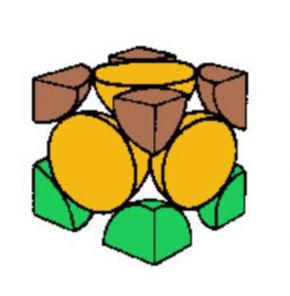
\includegraphics[width=.45\textwidth]{austenite_fcc_crystal_structure.jpg}
    \caption{An austenite fcc crystal structure [59].}
    \label{ch3:figure:austenite}
\end{figure}

\subsection{Pearlite} 
When the largest amount of carbon has occupied the interstices to form austenite at the critical temperature, the steel gradually cools at eutectoid temperature (723℃) on the iron-iron carbide equilibrium diagram, shown in Figure \ref{ch3:figure:equilibrium}. Thus, the carbon content is forced out of the solution [44]. During this cooling process, the austenite transforms into a combination of ferrite and another phase known as cementite, also known as iron carbide, which has the chemical composition of Fe3C [61]. The combination of ferrite and cementite is known as pearlite.  
For plain carbon steels, ferrite, cementite, and pearlite phases are the principal constituents of the microstructure, provided that they have been cautiously subjected to slow cooling to avoid the formation of the metastable phases. Consequently, it is significant to evaluate the nucleation and growth of these phases and to determine the factors which control their morphology [44]

\begin{figure}[H]
    \centering
    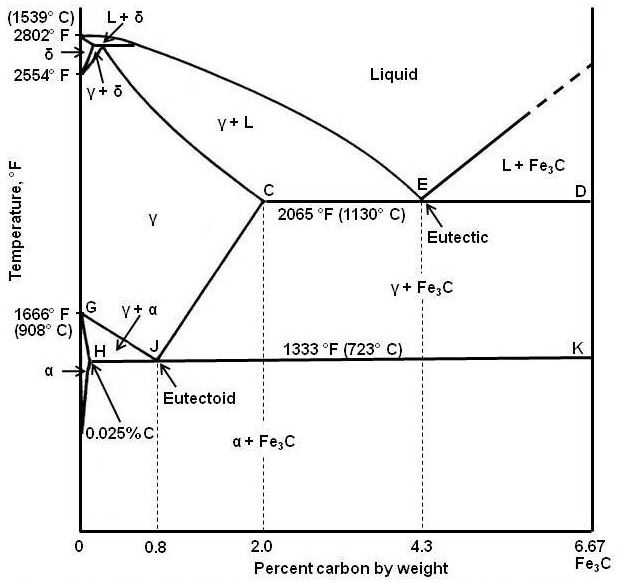
\includegraphics[width=\textwidth]{iron-iron_carbide_equilibrium_diagram.jpg}
    \caption{Iron-iron carbide equilibrium diagram showing the austenite ($\gamma$), ferrite ($\alpha$) and cementite (Fe3C) phase regions with eutectoid composition and temperature [61].}
    \label{ch3:figure:equilibrium}
\end{figure}

Cementite on its own has characteristics of ceramic materials, very hard and brittle, with low toughness and little resistance to crack initiation and propagation, which is unlike ferrite [59] As a result, pearlite may reveal more than one microstructure due to the alternating layers of ferrite and cementite. A fully pearlitic microstructure is significantly formed at the eutectoid composition of 0.78\%C, as shown in Figure \ref{ch3:figure:equilibrium} [30]. In contrast to cementite, the fully pearlitic steels have high strength, high hardness, and good wear resistance. However, they commonly suffer from poor ductility and poor toughness [30]. Figure \ref{ch3:figure:pearlite:microstructures} shows a microstructure fully pearlite steel and pearlite showing ferrite and cementite lamellae.

\begin{figure}[H]

\centering
\begin{subfigure}{.45\textwidth}
    \centering
    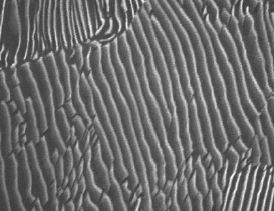
\includegraphics[height=5cm,width=\textwidth]{ferrite_and_cementite_lamellae_micrograph.jpg}
    \caption{}
\end{subfigure}
\begin{subfigure}{.45\textwidth}
    \centering
    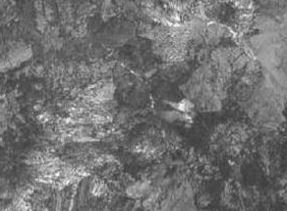
\includegraphics[height=5cm,width=\textwidth]{fully_pearlitic_steel.jpg}
    \caption{}
\end{subfigure}

\caption{Pearlite microstructures:  a) SEM micrograph of pearlite showing ferrite and cementite lamellae. 4\% picral etch. 10000x. b) Fully pearlitic steel showing the characteristic fine pearlite interlamellar spacing. 2\% nital + 4\% picral etch. 500x [30].}
\label{ch3:figure:pearlite:microstructures}
\end{figure}

\subsection{Ferrite-Pearlite}
Ferrite-pearlite is the common microstructural phase that makes most plain carbon steels. The microstructure and properties of these steels are distinguished, usually by the carbon content present and the size of the grains, as shown in Figure \ref{ch3:figure:austenite} [30]. However, as previously stated in section 3.6, carbon content has an impact on some properties of steel, thus it has a strong relationship with the tensile strength of ferrite-pearlite steels. As illustrated in Figure \ref{ch3:figure:properties}, carbon content has a direct relationship with the ultimate strength of ferrite-pearlite steels due to the gradual increase of ultimate tensile strength as a function of carbon content [62]. 
Pearlite has more carbon content on the microstructure, thus this is the main reason for the increase of the ultimate strength on ferrite-pearlite steels [59] Consequently, the strength of pearlite is much higher than that of ferrite [30]. In contrast, the yield strength of ferrite-pearlite steels is not dependent upon the carbon content. However, the ferrite matrix commonly governs the yielding in ferrite-pearlite steels. Ferrite matrix is regarded as a repeating phase in the microstructure of ferrite-pearlite, hence pearlite alone has a slight effect on the yielding behavior [30]. Figure \ref{ch3:figure:contents} shows the microstructure of ferrite-pearlite steels at two different carbon contents, to further understand the effect of carbon on steels.

\begin{figure}[H]

\centering
\begin{subfigure}{.45\textwidth}
    \centering
    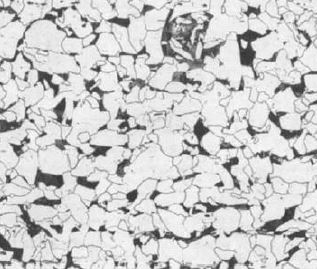
\includegraphics[height=.95\textwidth, width=\textwidth]{ferrite-pearlite_carbon_content_1.jpg}
    \caption{}
\end{subfigure}
\begin{subfigure}{.45\textwidth}
    \centering
    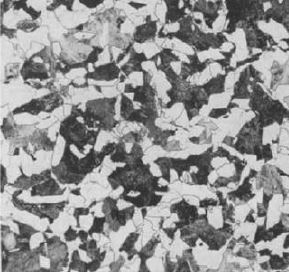
\includegraphics[height=.95\textwidth, width=\textwidth]{ferrite-pearlite_carbon_content_2.jpg}
    \caption{}
\end{subfigure}

\caption{Microstructure of typical ferrite-pearlite steels at two different carbon contents: a) 0.10\% C and b) 0.25\% C. 2\% nital + 4\% picral etch. 200x [30].}
\label{ch3:figure:contents}
\end{figure}
 
\begin{figure}[H]
    \centering
    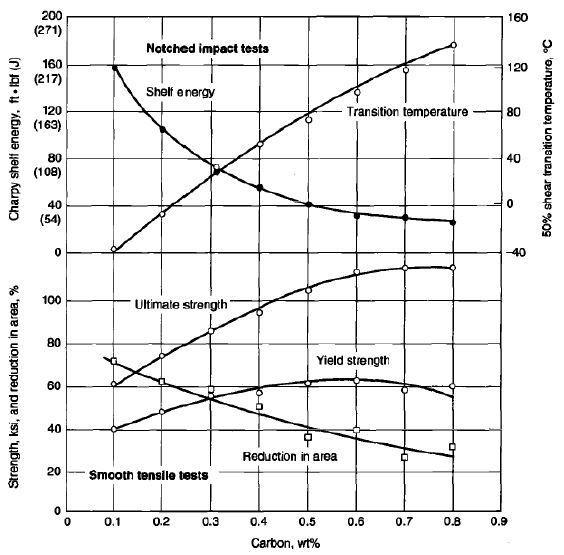
\includegraphics[width=.8\textwidth]{mechanical_properties_of_ferrite-pearlite_steels.jpg}
    \caption{Mechanical properties of ferrite-pearlite steels, as a function of carbon content [30]. }
    \label{ch3:figure:properties}
\end{figure}

\subsection{Martensite}
Martensite is a supersaturated solid solution of carbon in iron [30]. It is generally formed during the rapid cooling process when the waste carbon of the fcc austenite does not have time to diffuse out of the crystal structure and form cementite [59] Instead, the carbon content is 'trapped' in with the now almost pure iron, and is relatively forced into interstitial locations that are not large enough to accommodate the carbon atoms. Consequently, this distorts and strains the crystal matrix into a body-centered tetragonal (bct) structure, as shown in Figure \ref{ch3:figure:martensite}. Thus this forms a very hard phase known as martensite [30].
 
\begin{figure}[H]
    \centering
    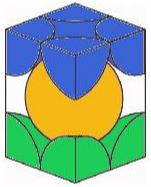
\includegraphics[width=.25\textwidth]{bct_crystal_structure_of_martensite.jpg}
    \caption{A bct crystal structure of martensite, which has larger gaps within the unit cell [59].}
    \label{ch3:figure:martensite}
\end{figure}

When the content of carbon is constantly increasing to higher levels, more carbon is frozen into the bct structure, further straining the crystal matrix. Thus this is the main reason for the hardness of martensite to increase a function of carbon content [59] In addition, the volume of the bct martensite structure is larger than that of the fcc austenite. Consequently, the transformation of fresh martensite is significantly compressed by the surrounding matrix [59]. A typical microstructure of martensite is shown in Figure \ref{ch3:figure:martensite:microstructures}.
The hardness of martensite can be significantly reduced by further heating the martensite. In such cases, the carbon content has the opportunity to diffuse out from the bct structure, reducing the distortion of the crystal matrix in that process, and thus reducing the hardness and increasing the toughness [44]. However, after the heat treatment process, the microstructure of ferrite and iron carbide is formed, which leads to the formation of tempered martensite [59]. Since the martensitic matrix is strained, it results in an increased amount of iron carbide nucleation sites in tempered martensite, which eventually leads to a more widespread distribution of iron carbide than seen in the lamellar (layered) structure of pearlite, shown in Figure \ref{ch3:figure:microstructure} [59] The bcc ferrite has a smaller volume compared to bct martensite, thus when martensite is tempered, some of the remaining martensite compression stresses from the austenite-to-martensite transition are mitigated [30].

\begin{figure}[H]
\centering

\begin{subfigure}{.45\textwidth}
    \centering
    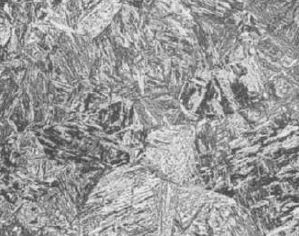
\includegraphics[height=6cm, width=\textwidth]{lath_martensite_microstructure.jpg}
    \caption{}
\end{subfigure}
\begin{subfigure}{.45\textwidth}
    \centering
    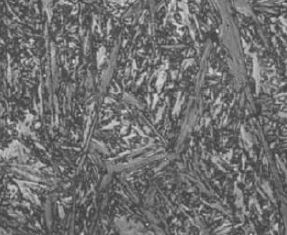
\includegraphics[height=6cm, width=\textwidth]{plate_martensite_microstructure.jpg}
    \caption{}
\end{subfigure}

\caption{Martensite microstructures: a) a typical lath martensite and b) a plate martensite. 4\% picral + HCl. 200x [30].}
\label{ch3:figure:martensite:microstructures}
\end{figure}

\subsection{Bainite}
Bainite is another possible microstructure that can form when austenite is cooled. It is typically the mixture of ferrite, cementite, and retained austenite. However, ferrite has an acicular morphology and the carbides are discrete particles, which is the main difference from the pearlite microstructure [30]. Retained austenite is the term given to austenite that does not transform to martensite during quenching [59] The cooling rate required to form bainite is much slower compared to the cooling rate needed to form martensite. As a consequence, carbon has the opportunity to diffuse out of the fcc austenite, thus allowing the formation of bcc ferrite.  
Bainitic microstructures have an excellent balance in terms of strength and ductility, which is useful in many applications. These are the results of a sufficient cooling rate that significantly increases the strength. The higher cooling rates required to produce bainite give the harder components of the microstructure enough energy to transform into a more rounded shape [59]. In this way, the hard microstructural constituents do not easily suffer to crack initiation and propagation as compared to flat and elongated.
Normally bainite has two morphologies as namely, upper bainite and lower bainite, which are shown in Figure \ref{ch3:figure:bainite:microstructures}. These two morphologies depend upon the temperature regions at which bainite was formed during the isothermal transformation [30]. The upper bainite is typically formed isothermally in the temperature range of 400-550 $^\circ C$, while lower bainite is also formed by an isothermal process in the temperature range of 250-400 $^\circ C$ [30]. Consequently, the iron carbide phase critically forms at the lath boundaries in upper bainite, while the carbide phase forms on certain crystallographic planes within the laths in lower bainite [59]. The lower bainite has higher strength and higher toughness compared to the upper bainite due to the fine acicular structure and the carbides within the laths. Generally, lower bainite has higher strength and higher toughness compared to upper bainite. This is due to the fine acicular structure and carbides possessed by lower bainite within the laths [30].
     
\begin{figure}[H]

\centering
\begin{subfigure}{.45\textwidth}
    \centering
    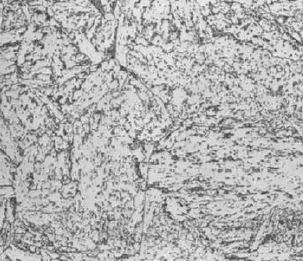
\includegraphics[height=.9\textwidth, width=\textwidth]{upper_bainite_microstruce.jpg}
    \caption{}
\end{subfigure}
\begin{subfigure}{.45\textwidth}
    \centering
    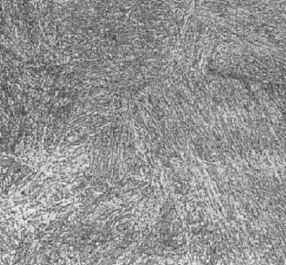
\includegraphics[height=.9\textwidth, width=\textwidth]{lower_bainite_microstructure.jpg}
    \caption{}
\end{subfigure}

\caption{Bainite microstructures: a) upper bainite and b) lower bainite in Cr-Mo-V rotor steel. 2\% nital + 4\% picral etch. 500x [30].}
\label{ch3:figure:bainite:microstructures}
\end{figure}

\subsection{Ferrite-Cementite}
When plain carbon steels are heated to temperatures slightly below the lower critical temperature, a ferrite-cementite microstructure that has a spheroidized shape as shown in Figure \ref{ch3:figure:spheroidized_steel} is significantly formed [30]. However, the spheroidized structure is commonly revealed after the formation of pearlite. During the spheroidization, the cementite lamellae of the pearlite change their morphology to result to form spheroids [30].
The critical and controlling factors during this process are the diffusion of carbon and portions of lamellae that should significantly dissolve and then diffuse to yield in the formation of a spheroid from the remaining portions of lamellae [30]. The ferrite-pearlite phase has several benefits in terms of the resulting properties. For example, fully spheroidized structures normally have enhanced machinability properties for most plain carbon steels [30].  Machinability of steels is one of the vital properties in the present study thus the formation of ferrite-cementite should be thoroughly evaluated and assessed.

\begin{figure}[H]
    \centering
    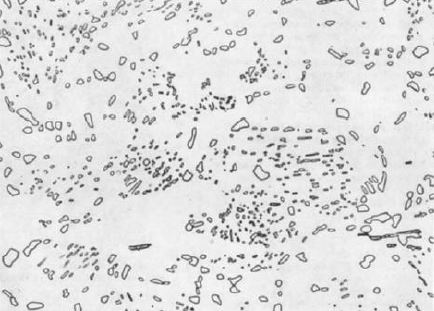
\includegraphics[width=.55\textwidth]{microstructure_of_fully_spheroidizel_steel.jpg}
    \caption{Microstructure of fully spheroidized steel. 4\% picral etch. 100x [30].}
    \label{ch3:figure:spheroidized_steel}
\end{figure}

\subsection{Ferrite-Austenite}
The ferrite-austenite are the two phases that are present in duplex stainless steels, see Figure \ref{ch3:figure:steel_phase}. The proportion of these two phases in duplex stainless steels in relatively equal. The duplex stainless steels can be altered to a completely ferritic structure. This is possible when they are melted and solidifies from the liquid phase[63].  However, as the materials significantly cool to room temperature, about half of the ferritic grains transform into austenitic grains [64]. Figure \ref{ch3:figure:duplex_microstructure} shows a combination of ferrite and austenite phases that forms one microstructure.
The combination of ferrite and austenite structures yields in several attractive properties. Consequently, duplex stainless steels are about twice as stronger compared to regular austenitic and ferritic stainless steel [64] The ductility of duplex steels is relatively fair, they however do not reach the excellent values of austenitic grades due to the different levels of nickel [30]. The stress corrosion resistance is another property that has made duplex stainless steels to be the extensively utilized family of stainless steels. 

\begin{figure}[H]
    \centering
    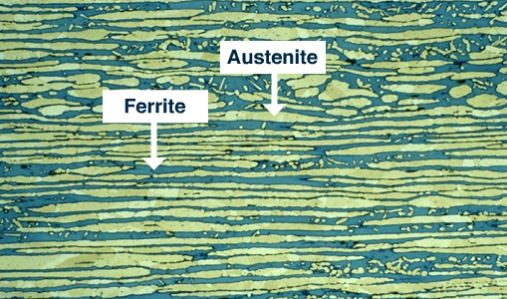
\includegraphics[width=.6\textwidth]{duplex_microstructure_that_has_yellow_austenitic_phase.jpg}
    \caption{Duplex microstructure that has yellow austenitic phase as “islands” surrounded by the blue ferritic phase [64].}
    \label{ch3:figure:duplex_microstructure}
\end{figure}

\section{Characterization of defects} 
While the microstructure of steels critically determines the resulting properties, they may still have a variety of imperfections known as defects and discontinuity. Both material discontinuity and crystal defects have diverse effects on the deformation behavior and some of the physical and chemical properties of steels [58]. Hence it is of great significance to determine the nature and quantity of the crystal defects present in a steel material. 
There are numerous methods they have been extensively utilized to characterize the defects in steels. However, according to some researchers, the Transmission Electron Microscopy (TEM) technique is more suitable to characterize defects on steels [43, 44]. Besides, the TEM method has been proven to be reliable on numerous occasions. In any metallic material crystal defects can occur, these defects may include, point defects (vacancies, interstitial atoms), line defects (dislocations), planar defects (stacking faults, twin boundaries), and volume defects (voids, cavities). One of the objectives of the present study is to improve the properties of steels based on the understanding of microstructure morphology. Thus, the characterization of vacancies and dislocation defects is also of interest.

\subsection{Vacancies} 
 In almost every instance, individual vacancies cannot be seen on TEM, due to the size and complications that are usually encountered. However, their aggregation into voids, resulting in the formation of dislocation loops in quenched steels, helps in estimating the vacancy concentration. In this way, the dislocation loops are significantly characterised, which then makes it possible to determine whether they are formed from vacancy condensation or interstitial atoms [58].

\subsection{Dislocations}   
This defect is commonly divided into two types, screw and edge dislocation. The complications arise when characterizing the type of dislocation that is present in steels [60]. However, this is conveniently achieved by using the extinction (invisibility) criterion g.b = 0, where g is the reciprocal lattice vector, and b is the burgers vector. By properly orientating the specimen, a dislocation will become invisible, and this can occur at more than one g value. The equation can nonetheless be manipulated by simply putting the determination of two (or more) of these g values, which then enables calculating b [58]. 
Many experimental studies have been conducted in order to ease and improve the characterization of crystal defects [43-44, 46]. Despite this, Suryanarayana [58] validated that TEM remains a suitable technique for characterizing crystal defects in steels. Moreover, TEM enables the determination of disorientation between grains (for both low-angle and high-angle grain boundaries), the fault vector in stacking faults, the extent of coherency, or incoherency between two phases, the sizes and volume fractions of precipitates, and many other features [58].

\section{Effects of heat treatment on steels} 
Heat treatment is an industrial process that is commonly used to improve the existing properties of the metals, especially steels. To be precise, it is often used to enhance mechanical, physical, and sometimes chemical properties [65]. The heat treatment process modifies the microstructure of the steels, thus altering the resulting properties. The role of each microstructural constituent in comprehensively presented in Table C.5 on appendices. In recent years several methods have been developed to enhance the properties of engineering materials, especially for liquid storage facilities. Approaches like thermochemical and thermomechanical are examples of such techniques [66]. However, the heat treatment process has been a sensible approach for the optimization of steel properties.
Normally, the first step in heat treatment of steel is to effectively heat the steel to some temperature at or above the critical range to form austenite and  [65]. However, to fully comprehend the heat treatment process of steels, it is crucial to first understand the phase diagram for the steel of interest. Heat treatment comprises of several subsequent processes that are all critical. Various heat treatments are normally based on the subsequent cooling and reheating of the austenitized steel [66].  For the present research work, only the relevant heat treatment processes will be discussed.

\subsection{Annealing}
The ductility of steels or any metallic material is normally enhanced by the annealing process. This process involves heating the steels to a predetermined temperature and then slowly cooling it to room temperature in a furnace [66]. However, enhancing the ductility of the steel results in a reduction in brittleness. Sometimes annealing process can be utilized to improve the machinability of steels [67]. As a consequence, annealing is a vital process for liquid storage facilities due to the demand for ductility and ease of machinability during the fabrication process. The full annealing temperature cycle is shown in Table D.1 on appendices, which includes the hardness rage on steel after annealing. 
Annealing is a broad process that involves several thermal cycles, which are classified based on the maximum level of temperature reached during the heating of the steel [66]. The thermal cycles usually involve subcritical, intercritical, and full annealing. Appendix 2.1 indicates the recommended temperatures and cooling cycle for full annealing of various carbon steel forgings [66]. 

\subsection{Normalizing}
The purpose of normalizing is very broad and normally depends upon the history of the steel, the cycle of heating, and cooling practiced. However, this process is commonly used to achieve the desired hardness and strength of the steel [66]. Therefore, it can increase or decrease these properties, depending on the objectives. 
Normalizing is sometimes known for overlapping the function of other types of heat treatments, such as annealing, hardening, and stress relieving [66]. This is due to multiple properties it normally improves simultaneously, which can be individually achieved by each other heat treatment processes. Normalising can produce harder and stronger steel and also improves machinability [65]. However, in the normalizing process, the cooling is not performed under equilibrium conditions, thus there are often deviations from the phase diagram predicted structures [66].  For steels that are normally used for the construction of liquid storage facilities, normalizing is essential to achieve the desired strength and hardness, as well as the improved machinability.

\subsection{Tempering}  
Almost all steels are too brittle in the quenched martensitic condition for most applications, especially storage facilities. This is due to high residual stresses that are commonly induced as the result of the martensite transformation [65]. Consequently, tempering always follows the hardening or normalizing process in order to relieve the residual stresses and relax the steel. 
Tempering is a heat treatment process that involves heating of the steel to the temperature below the lower critical temperature [66]. This results in relieving the residual stresses, and the enhancement of the ductility and toughness of the steel. In most heat treatment processes, there is usually a sacrifice of other properties to obtain others. As a consequence, in the tempering process, there is a sacrifice of hardness and strength. As the tempering temperature is constantly increased, the hardness decreases, while the toughness increases [66]. Various types of tempering are known to date, austempering and martempering are the commonly used processes.

\subsection{Quenching}  
The rate of cooling any metallic material is vital and has an impact on the resulting properties. Quenching is the process of cooling the steel, usually at a rapid rate, to produce a martensitic transformation [66]. The rate of cooling has different effects on different metals, in ferrous alloys, the rapid rate will result in a harder metal, while in non-ferrous alloys, the softer metal will be produced [65]. The rapid rate of cooling usually hardens steel. Therefore, in order to achieve softer steel, a slower rate of cooling should be applied. However, this, of course, varies with the type of steel. 
Quenching can be achieved in numerous ways, commonly by forced air or other types of gases. Liquids such as water and oil can also be utilized to quench steels due to their better thermal conductivity [66]. There are three stages of cooling during the quenching process, and all are closely related to the cooling medium being used. Vapour is the first quenching medium that is applied at the steel surface, and during this stage, the cooling process is relatively slow. When the metal has cooled enough, and the vapor film is no longer stable, the second stage then takes place, which is wetting of the surface of the steel. This is usually the rapid stage of cooling the steel. Finally, liquid cooling commences when the surface temperature of the steels finally reaches the boiling point of the liquid to halt the formation of vapor [49-50]. However, this is commonly the slowest stage of cooling.
Recently, most of the researchers have been interested in understanding the relationship between heat treatments, microstructure, and mechanical properties [49, 51, 54]. Mampuya et al [65] investigated the effect of heat treatment on the microstructure of duplex stainless steel 2205. They further reported that the transition of austenite and ferritic phases often results in the critical changes in the hardness of the specimen when air-cooled. While there is a slight change in the hardness when it is water or oil cooled. Ding et al [70] conducted an experimental study to understand the effect of slow-cooling heat treatment on the mechanical properties of high strength steels. Their results indicated that the slow-cooling heat treatment can effectively reduce the yield and ultimate strengths of high strength steels. Essoussi et al [71] reported that the strength and elongation of AISI 304 austenitic stainless steels can be improved by quenching without tempering, while the hardness will relatively decrease during this process.
There is a lack of research on the effect of heat treatment on the corrosion properties of steels. However, some researchers have made a significant effort to thoroughly understand the relationship between corrosion and heat treatment processes [51, 52]. The corrosion resistance of steels is largely dependent upon the composition and microstructures [69]. The microstructures could nonetheless be improved by the process of heat treatment. Sarkar et al [68] investigated the effect of heat treatment on the microstructure, mechanical, and corrosion properties of stainless steel. The investigation showed that the retained austenite is more for specimens without solution annealing, which increases the tensile strain and decreases the hardness and wear rate. In an effort to enhance the corrosion resistance of martensite stainless steel, Wang et al [69] conducted numerous experiments and they reported that the austenite phase disappears and new duplex particles accelerated after solution treatment and aging treatment, which decreased the pitting corrosion. 
One of the objectives of the present research work is to improve the corrosion resistance of duplex stainless and mild steels in a corrosive atmosphere. Consequently, all these previous studies and relevant literature is used as a benchmark for the present study. Experimentally and theoretically, they provide comprehensive guidance in terms of optimizing the materials used for constructing AFFF storage facilities.

\section{Polyethylene plastics}
Plastics also known as polymers have become a major class of engineering materials. Polymers are substances whose molecules have high molar masses and are composed of relatively large number repeating units. There are both naturally occurring and synthetic polymers [72]. They offer several beneficial properties (mechanical, physical, chemical and optical) when utilised for certain industrial applications [73]. In contrast to metals, polymers are generally characterised by lower density, strength, elastic modulus, thermal and electrical conductivity, high corrosion resistance, and cost [72]. Thus, this is the reason for the rapid increase on plastic processing on annul basis. In addition, they are the preferred materials over metals in nowadays for numerous industrial applications. However, their setback to date is they are a waste that affects the environment if no longer in use. Nonetheless, there have been developments over the years that are aiming to rectify this issue, with the notable one being recycling.  
There are many plastic materials that fall under polymer tree. However, for the purpose of the present study polyethylene (PE) plastics will be discussed. This is due to the growing demand of this material for manufacturing liquid storage facilities. PE is undoubtable the most popular plastic material in the world. It is a commodity material, which statically accounts for about 70\% of the plastic family [72].  PE is a thermoplastic in nature and therefore it can be reprocessed repeatedly, thus this is the reason it is easily available at relatively low cost and can be easily processed [74]. Moreover, it can be utilised for diverse industrial applications. 
PE is often classed by the density it contains. Therefore, there is a Low-Density Polyethylene (LDPE) ($0.910 < density < 0.925$), Medium-Density Polyethylene (MDPE) ($0.926 < density < 0.940$), and High-Density Polyethylene (HDPE) [75]. Consequently, changing the density of the PE will results in altering the properties. The effect of changes in density, melt index, and molecular weight distribution on the properties of PE are tabulated in Table E.7 on appendices. 
HDPE is commonly used in the manufacturing of chemical or liquid storage facilities, due to the seamless final product that is produced, for greater strength and corrosion resistance, thus it is off great importance in the present study. HDPE is a thermoplastic material composed of mainly carbon and hydrogen atoms joined together to form a high molecular weight products as shown in Figure \ref{ch3:figure:molecular_chains} [75]. Methane gas is converted into ethylene then, with the application of heat and pressure it is further converted to polyethylene. The polymer chain may be 500,000 to 1,000,000 carbon units long. The longer the main chain, great the number of atoms [75]. As expected, the properties of HDPE or any plastic material depends upon the arrangement of the molecular chains. 
               
\begin{figure}[H]
\centering

\begin{subfigure}{.3\textwidth}
    \centering
    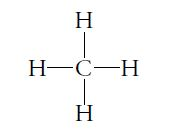
\includegraphics[width=\textwidth]{methane_molecular_chain.jpg}
    \caption{Methane}
\end{subfigure}
\begin{subfigure}{.3\textwidth}
    \centering
    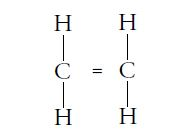
\includegraphics[width=\textwidth]{ethylene_molecular_chain.jpg}
    \caption{Ethylene}
\end{subfigure}
\begin{subfigure}{.65\textwidth}
    \centering
    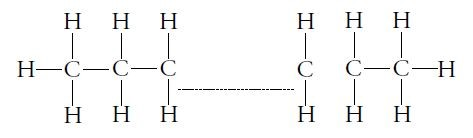
\includegraphics[width=\textwidth]{polythylene_molecular_chain.jpg}
    \caption{Polyethylene molecular chain}
\end{subfigure}

\caption{a) Methane gas, b) ethylene and c) polyethylene [75].}
\label{ch3:figure:molecular_chains}
\end{figure}

\subsection{Cross-linked polyethylene (XLPE) material}

Since early 1030’s many researchers have been making efforts in obtaining a PE with specific chemical, mechanical, and thermal characteristics for the fabrication of complex-shaped products, or for use in adverse environmental conditions [74]. In general, plastic is a light and weak substance that easily melts when exposed to heat. However, altering the carbon atoms within the structure changes this perspective. To be precise, cross-linking the carbon atoms within the structure usually transforms such material into a superior material that may be resistant to temperature, pressure, corrosion, and that can be used in a variety of applications [76]. Crosslinking is known as a process in which carbon atoms of same or different polyethylene chains are joined together to form the three-dimensional network structure [74].
The crosslinking technique was first discovered in late 1960’s by the European scientist known as Engel [76]. The introduction of cross-linked polyethylene (XLPE) was another milestone in the plastic era. As a consequence, when PE is cross-linked, it is advantageously employed in the manufacturing of storage facilities due to the advanced resulting properties. In fact, the fundamental way to enhance material properties such as impact strength, chemical resistance, and thermal characteristics is via cross-linking [77]. Cross-linking will however change the nature of polymer from thermoplastic to thermosetting polymer, thus yielding to a non-melting and more durable polymer matrix [57]. Crosslinking method is easily achieved in branched polymers. From the branched HDPE it is convenient to crosslink the polymer. However, this is a long and tiring process as compared to LDPE.
Since HDPE has a linear molecular structure, therefore crosslinking this type of polymer requires a special attention as compared to LDPE. Figure \ref{ch3:figure:hdpe} and \ref{ch3:figure:ldpe} shows the process of branching HDPE and LDPE respectively.
 
\begin{figure}[H]
    \centering
    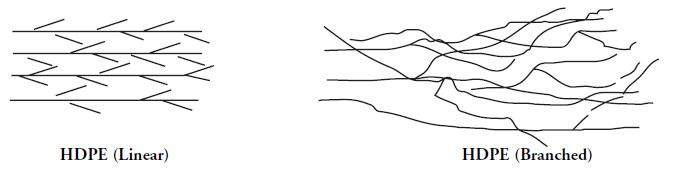
\includegraphics[width=\textwidth]{linear_and_branched_hdpe.jpg}
    \caption{Linear and branched HDPE [75].}
    \label{ch3:figure:hdpe}
\end{figure}

\begin{figure}[H]
    \centering
    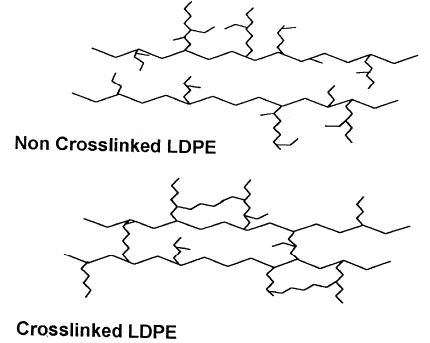
\includegraphics[width=.6\textwidth]{crosslinked_and_non_crosslinked_ldpe.jpg}
    \caption{Crosslinked and non-crosslinked LDPE. [74].}
    \label{ch3:figure:ldpe}
\end{figure}

Over the past decades, there have several crosslinking methods that have been developed. However, to date, there are two tested methods that are used to crosslink polymers, chemical and radiation (physical) methods [57, 59]. These two methods are unique in their own way and are often utilized for a specific purpose. They usually depend upon the state (molten or solid) of the polymer during crosslinking and the type of activator used to promote crosslinking [74]. Figure \ref{ch3:figure:crosslinking_methods} illustrates the available crosslinked methods in detail, as discussed above.

\begin{figure}[H]
    \centering
    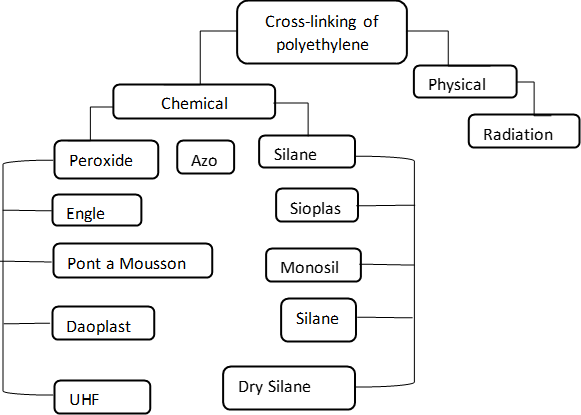
\includegraphics[width=.75\textwidth]{methods_available_for_crosslinking_polyethylene.png}
    \caption{Methods available for crosslinking polyethylene [78].}
    \label{ch3:figure:crosslinking_methods}
\end{figure}

\subsubsection{Chemical processes}
This is an extensively used method for crosslinking polymers. In order for the method to work as desired, a chemical substance usually peroxide or silane is required to significantly activate the links in the polymer chain, thus it is known as a chemical process [76]. During chemical process, the crosslinking takes place through direct carbon-to-carbon bonds. An alternative may be through the chemical bridges that connect various polyethylene molecules [74].  
In recent years, most researchers have been interested in knowing the crosslinking method that yields to quality thermoplastic. The recent relevant literature suggests that the intensity of crosslinking in thermoplastic resin usually varies with the crosslinking process. Chemical crosslinking using peroxide significantly results in highest and uniform degree of crosslinking as compared to radiation process [57, 59]. Tamboli et al [76] experimentally investigated the difference in degree of crosslinking polymers using chemical and radiation process. The outcome was that radiation crosslinking yields between 34-75\% degree of crosslinking. In chemical crosslinking method, peroxide gives much high degree of crosslinking (up to 90\%), while silane-based crosslinking can be 45-70\% degree of crosslinking.

\paragraph{Peroxide processes}
 Peroxide crosslinking process has been utilised for nearly over 40 years and is the most common crosslinking process of thermoplastics, especially polyethylene. In this method, the organic peroxide is used as the initiator. In most cases, organic peroxide is used its original unprocessed structure [76]. It is important to note that this process only occurs when the thermoplastic is in molten state. In addition, the process is a carbon-based chemical that includes a minimum of two oxygen atoms that are bonded together (-O-O-). The general formula is:  

 \begin{equation}
    R^1-O-O-R^2
 \end{equation}

Where: R1 and R2 values can be aryl, alkyl, or acyl groups and O being the two oxygen atoms which are bonded together. The alkyl peroxides significantly produce the most reactive free radicals thus they are the most used peroxides for crosslinking [74]. Figure \ref{ch3:figure:crosslinking_process} shows the entire schematic representation of crosslinking polyethylene using the peroxide substance. Peroxide process has the advantages of producing high thermal stability products due to the C-C bonds, however, this is achieved relatively high costs [78].

\begin{figure}[H]
    \centering
    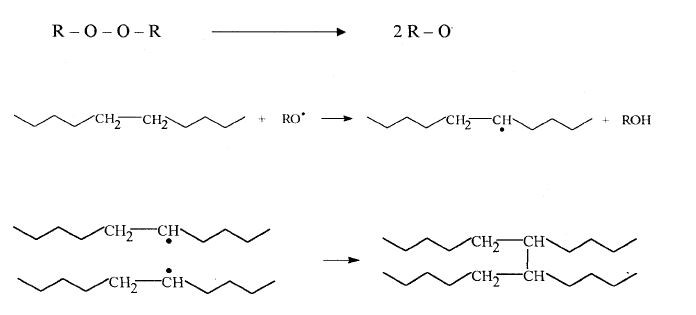
\includegraphics[width=.9\textwidth]{process_of_crosslinking_using_the_organic_peroxide_as_the_initiator.jpg}
    \caption{Process of crosslinking using the organic peroxide as the initiator [76]. }
    \label{ch3:figure:crosslinking_process}
\end{figure}

\paragraph{Silane processes}
For this process to be possible, the crosslinking is significantly activated by silane coupling agents, which react with many chemicals, including polymers, through typical organic chemistry reactions. The organ silane molecule critically includes a central silicon atom (Si) bounded to two different categories of groups (vinyl and alkoxy), which usually displays different reactivity [74]. Both these groups are vital in the process of crosslinking. The vinyl groups usually allow silane grafting to the PE and alkoxy grounps generate a three-dimensional network of siloxane linkages in the presence of water or moisture (through condensation or hydrolysis). 

In contrast to peroxide process, the PE is cross-linked in the crystalline state in silane process. Thus, the uses of silanes result in the formation of siloxane (Si-O-Si) bridges, which are less rigid than carbon-to-carbon (C-C) bonds produced in the peroxide process. The silane process is shown in Figure \ref{ch3:figure:reaction} in a two-step process, starting from grafting of silane on PE to condensation (crosslinking). At first, silane is grafted on PE, then the condensation takes place yielding in crosslinking. One of the advantages of silane process is that it can be achieved at room temperature and at relatively low cost. 

\begin{figure}[H]
\captionsetup[subfigure]{justification=raggedright}

\centering

\begin{subfigure}{.9\textwidth}
    \centering
    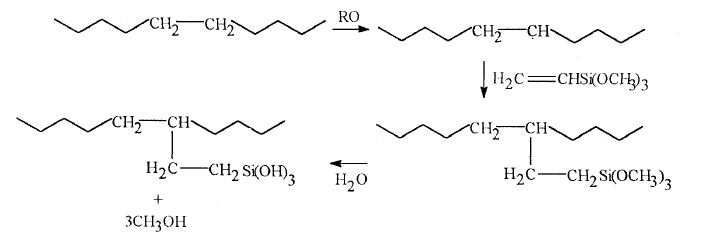
\includegraphics[width=\textwidth]{grafting_of_silane_on_pe.jpg}
    \caption{Grafting of silane on PE}
\end{subfigure}
\begin{subfigure}{.9\textwidth}
    \centering
    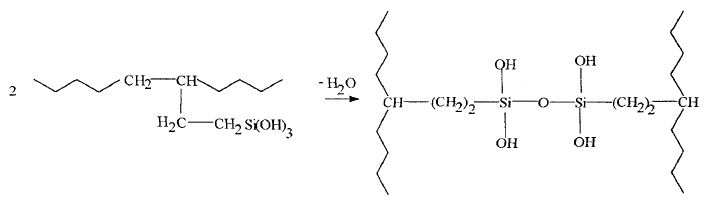
\includegraphics[width=\textwidth]{condensation.jpg}
    \caption{Condensation (crosslinking)}
\end{subfigure}

\caption{Silane grafted polyethylene crosslinking reaction [74].}
\label{ch3:figure:reaction}
\end{figure}

\paragraph{Radiation (physical) processes}
In contrast to chemical processes, radiation processes do not necessarily require any addition of any sort of chemicals in the original compound of PE. In radiation method, crosslinking is significantly achieved by free radical mechanism, which is generated in radiations polymer chain using high energy [76]. As a consequence, two or more chains will join together where the free radical is generated. Figure \ref{ch3:figure:radiation} shows a schematic process of crosslinking PE by radiation. 
The involvement of high energy radiation on polymeric materials can critically produce crosslinking or cause a degradation in the main chain, which is termed as ‘scission’ [79]. In this way, both chain scission and crosslinking occur simultaneously and competitively. However, the dominance of one or other may significantly depend upon several factors such as sensitivity of the polymer to radiation, irradiation dose, and polymer radiation environment [79]. To be precise, in the presence of oxygen (O2) scission is relatively dominant over crosslinking, while in an environment that contains other gases such a nitrogen (Ni), crosslinking is normally dominant [76]. However, the changes and chemical properties of the finished product depend mostly on the efficiency of crosslinking reaction and its relative ratio with degradation [79]. For AFFF storage facilities chemical properties of cross-linked polymer are of great important. This is due to the uses of AFFF, as its chemical composition should not be influenced by the holding storage facility.  

\begin{figure}[H]
\captionsetup[subfigure]{justification=raggedright}

\centering

\begin{subfigure}{.9\textwidth}
    \centering
    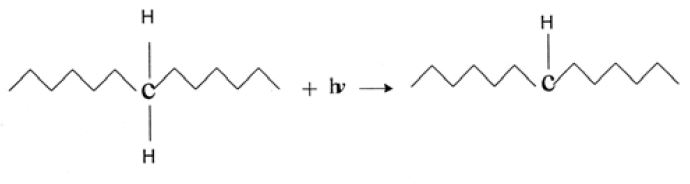
\includegraphics[width=\textwidth]{polyethylene_energy_radiation.jpg}
    \caption{}
\end{subfigure}
\begin{subfigure}{.9\textwidth}
    \centering
    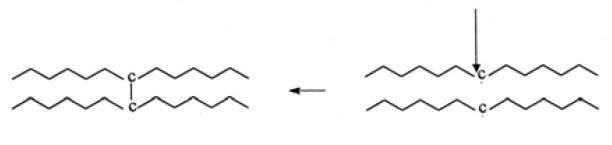
\includegraphics[width=\textwidth]{resulting_crosslinked_pe.jpg}
    \caption{}
\end{subfigure}

\caption{a) Polyethylene energy radiation and b) the resulting crosslinked PE [76].}
\label{ch3:figure:radiation}
\end{figure}

Mathematically, the scission and crosslinking can be related in order to estimate the probability between them. This probability can be expressed as a ratio that is given by the following equation.

\begin{equation}
    \frac{\beta}{\alpha}=\frac{1}{2}\frac{G(S)}{G(X)}
\end{equation}

\noindent Where, \\
$\alpha\ is\ a\ probability\ of\ crosslinking\ of\ chains\ after\ one\ electron\ volt\ of\ energy\ absorbed.$ \\
$\beta\ is\ a\ probability\ of\ chain\ scission\ after\ one\ electron\ volt\ of\ energy\ absorded.$ \\
$G(X)\ is\ a\ number\ of\ crosslinking\ per\ 100eV\ of\ radiant\ energy\ absorbed.$ \\
$G(S)\ is\ a\ number\ of\ scission\ per 100eV\ of\ energy\ absorbed.$ \\

The typical G(X) and G(S) values are listed in Table E.9 on appendices. \\

According to several scientists the bond energy for breaking of C-H bond is typically 364Kj/mol [76]. Therefore, the electron beam having sufficient energy to break C-H bond is normally suitable for crosslinking rather than scission [76]. The technique of crosslinking PE by radiation normally involves the four main variables. 

\begin{itemize}
    \item The type of radiation and its sources.
    \item The nature of PE structure to irradiated.
    \item Mechanism and theories of reaction.
    \item The properties of the network formation, especially physical, chemical, and mechanical. 
\end{itemize}

\subsection{Environmental Stress Crack Resistance (ESCR)}
AFFF solution contains sensitive chemicals within its composition. Therefore, under certain temperature and stress conditions, the PE material may begin to crack sooner than expected due to the presence of chemicals contained in AFFF solution. It has been experimentally proven that storage facilities containing liquids that are chemically free do not suffer to cracks as much as those containing chemical liquids. This phenomenon is known as the environmental stress crack (ESC). One of the objectives of the present work is to assess and evaluate the chemical resistance of XLDE in the presence of AFFF solution. The test methods that are usually utilised to evaluate ESC and other substances are provided in Table E.8 on appendices. 
All engineering materials that are suitable for storing liquids containing chemicals, are critically evaluated against ECS. For PE, normally the stress cracking agents are polar materials such as alcohols, detergents, halogens and aromatics [75]. AFFF may be thought of as a detergent due to the bubbles it creates during utilisation. Consequently, it definitely causes problems to PE polymers. The property of a material to resist ESC is called environmental stress crack resistance (ESCR) [75]. Researchers have been working on understanding the mechanism of ESCR, however, to date it is not entirely understood. In most instances, failures of PE polymers that are caused by ESC tend to be due to the development of cracks in area tensile stress which gradually grow and propagate over time [76]. 
Over the past years, there have been several efforts made in order to avoid ESC. Therefore, using an appropriate resin formulations of ESCR materials, designing the geometric appropriately, carefully using the manufacturing controls that prevents occurrence of severe stress risers, and limiting stresses and strains during the storage facility installation, all these are usually sufficient to avoid ESC [75]. Moreover, PE polymer may be cross-linked to improve the chemical properties and thus resist cracking.  With this regard, it is vital to test the compatibility of PE, especially XLPE with AFFF concentrate in order to avoid unexpected circumstances during fire conditions. To date, there are over 40 different ESCR test methods that are used to determine the chemical resistance of various materials. The standard test that is currently used in the industry of polyethylene is bent-strip test [75]. The method is normally used to assess the performance of polyethylene cable insulation but can be cautiously used to evaluate the performance of XLPE storage facilities in the presence of AFFF concentrate. The bent-strip test is shown in Figure \ref{ch3:figure:bending_apparatus}. Where the specimen is immersed into a surfactant of interest, and the time to failure is noted. The results are reported using the notation $F_{xx}$, where xx is the percentage of samples that has been tested.
 
\begin{figure}[H]
    \centering
    \includegraphics[width=.8\textwidth]{three_point_bending_apparatus_for_testing_escr.jpg}
    \caption{Three point bending apparatus for testing ESCR under constant strain. [80]}
    \label{ch3:figure:bending_apparatus}
\end{figure}

Research shows that the density of the PE polymer plays a critical role towards ESCR. For PE resins of the same molecular weight, the lesser the density, the greater the ESCR. The greater the proportion of crystals, the greater the density and the brittleness of the resin, which causes a rapid crack initiation [75]. However, since the phenomenon of ESC is not fully understood, then the density alone is inadequate to predict the ESCS. 

\section{Conclusions}
This chapter discussed the engineering materials investigated in the present study. Both metals and plastics materials were closely assessed. The previous research was studied; this was used as a benchmark in this research. The atomic bonding, cross-linking methods, properties of interest, microstructure, and heat treatment processes are investigated. Properties of most materials depend upon the microstructure. Consequently, heat treatment processes are vital when improving these properties.
PE plastics are rapidly replacing metals nowadays. They have several advantages over metal, as they are light in weight, resistant to corrosion, durable, and relatively affordable. These plastics are often classified by the density they possess. In this chapter, the environmental stress cracking resistance of these plastics was discussed. To alter the properties of PE, a cross-linking method was opted. To date, this is an effective method to avoid the phenomenon of ESC.
The next chapter discusses and compares the various methods of constructing the storage facilities for AFFF concentrate. The methods used to test the compliance of these storage facilities are discussed. Both national and international design standards are considered.

\chapter{Experimental set up}
\section{Introduction}
In this chapter, the aim of the experiment, the experimental procedure, the materials, the analysis of samples, and the detailed experimental methods employed are all concisely described. The analysis of the methods and the testing standards utilized are presented. These include the microstructural analysis, environmental stress cracking tests, and corrosion analysis of the three materials of interest, which are mild steel, stainless steel, and HDPE. All the parameters used are discussed and shown with the safety precautions being followed throughout the experiments. After AFFF solution has been exposed to various engineering materials, the composition and other vital performance parameters are critically analyzed.

\section{Aim of the experiment}
The experimental work aims to evaluate and assess the impact and compatibility of the storage facility (engineering materials) on the composition of AFFF, hence performance parameters. 

\section{Methodology}
Samples of stainless-steel, mild steel, and HDPE together with AFFF solution were carefully prepared. A guillotine machine was used to cut the material sheets into desired shapes and sizes. All the material sheets were cut to the same sizes and shapes for a fair comparison. A total of 5 samples were used during the experiments. These sample materials were exposed to natural environmental conditions, with another sample of mild steel being exposed to seawater for 60 days. All the samples were then immersed and soaked in 3\% proportion of AFFF solution for further 120 days. Fourier transform infrared spectroscopy (FTIR), Transmission electron microscopy (TEM), Dynamic Light Scattering (DLS), and Inductively Coupled Plasma (ICP) wet analysis were performed on sample materials. This was done to analyse the composition, properties and stability of AFFF solution after being exposed to these materials. 
During the tests, clean sample materials and AFFF solution from the manufacturer were used as a benchmark and their properties were compared to the exposed material to deduce any vital changes occurred. All the findings were carefully recorded and analysed. However, it should be noted that the objective was to analyze the AFFF solution. The experimental procedure followed for all the samples is presented in the flowchart in Figure \ref{ch4:figure:procedure}. 

\begin{figure}[H]
\centering

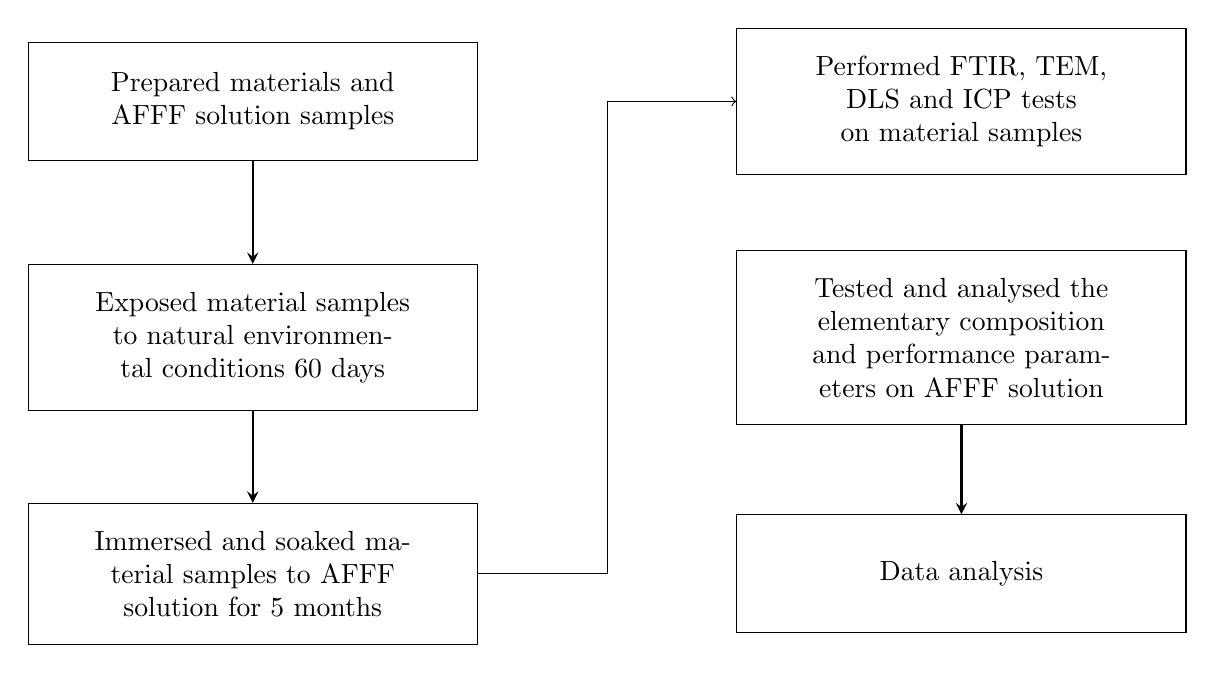
\begin{tikzpicture}[node distance=3cm]
    \tikzstyle{block} = [rectangle, minimum height=1.5cm, inner sep=1em, text centered, text width=5cm, draw=black]
    \tikzstyle{arrow} = [thick, ->, >=stealth]

    \node (prepare) [block] {Prepared materials and AFFF solution samples};

    \node (expose) [block, below of=prepare] {Exposed material samples to natural environmental conditions 60 days};

    \node (immerse) [block, below of=expose] {Immersed and soaked material samples to AFFF solution for 5 months};

    \node (perform) [block, right of=prepare, xshift=6cm] {Performed FTIR, TEM, DLS and ICP tests on material samples};

    \node (test) [block, below of=perform] {Tested and analysed the elementary composition and performance parameters on AFFF solution};

    \node (analyse) [block, below of=test] {Data analysis};

    \newcommand*{\connector}[4][]{
        \draw[#1] (#3) -| ($(#3) !#2! (#4)$) |- (#4);
    }

    \draw [arrow] (prepare) -- (expose);
    \draw [arrow] (expose) -- (immerse);

    \connector[->, black]{0.5}{immerse}{perform}

    \draw [arrow] (test) -- (analyse);

\end{tikzpicture}

\caption{Typical experimental procedure}
\label{ch4:figure:procedure}
\end{figure}

\section{Material description}
On the present experiments, 3, 4 and 5mm sheets of duplex stainless steel, mild steel and HDPE respectively were selected as the materials of interest. The sample sheets were scribed to ease and ensure that the cut sizes are precise during the cutting stage. The cut samples were further cut to three small pieces for accurate testing and the average results were considered. This was also done to accommodate the percentage errors and external factors which may have occurred during the experimental setup. Glass beakers of 800ml in volume were prepared to fill the 3\% proportion of AFFF solution and immerse the material samples. 

\section{Sample preparation}
\subsection{Experimental matrix}

\begin{table}[H]

\centering
\begin{tabular}{m{.25\textwidth} m{.25\textwidth} m{.4\textwidth}}
    \hline
    Material & Instrument & Analyses \\
    \hline
    AFFF solution & FTIR & Functional groups \\
    & TEM & Particle size and shape \\
    & & HR imaging \\
    & & Electron diffraction images \\
    & DLS & Particle size distribution \\
    & ICP & Elementary identification \\
    \hline
\end{tabular}

\caption{Experimental matrix with AFFF solution.}
\end{table}

\subsection{Material plates} 
The sheets of stainless steel, mild steel, and HDPE respectively were prepared for the experiments. These sheets required to be cut to the desired shapes and sizes so that they can fit in beakers filled with AFFF solution. The scriber was used to scribe the precise sizes and the shapes to be cut. This was done at the Durban University of Technology (DUT) manufacturing workshop, using a guillotine cutting machine. The prepared material samples can be seen in Figure \ref{ch4:figure:stainless_steel}, \ref{ch4:figure:mild_steel} and \ref{ch4:figure:hdpe}.
 
\begin{figure}[H]
    \centering
    \includegraphics[width=.55\textwidth]{duplex_stainless_steel_sample.jpg}
    \caption{Duplex stainless steel sample.}
    \label{ch4:figure:stainless_steel}
\end{figure}
 
\begin{figure}[H]
    \centering
    \includegraphics[width=.55\textwidth]{mild_steel_sample.jpg}
    \caption{Mild steel sample.}
    \label{ch4:figure:mild_steel}
\end{figure}

\begin{figure}[H]
    \centering
    \includegraphics[width=.55\textwidth]{hdpe_sample.jpg}
    \caption{HDPE sample}
    \label{ch4:figure:hdpe}
\end{figure}

\subsection{The cutting process}
The prepared samples were cut to the sizes of 60mm x 100mm using a guillotine machine. It can be seen in Figures \ref{ch4:figure:stainless_steel}, \ref{ch4:figure:mild_steel} and \ref{ch4:figure:hdpe} that the samples were firstly scribed before being cut to ensure the precision. Stainless steel and mild steel were cut using a guillotine that can cut up to a thickness of 5mm. In contrast HDPE was cut in guillotine that can cut up to 3mm thickness, it is not hard as the two steels. Figure \ref{ch4:figure:5mm_guillotine} and \ref{ch4:figure:3mm_guillotine} shows the two guillotine machines that were used to cut the samples.
 
\begin{figure}[H]
    \centering
    \includegraphics[width=.4\textwidth]{5mm_guillootine_machine.jpg}
    \caption{Guillotine machine that cuts up to 5mm thickness.}
    \label{ch4:figure:5mm_guillotine}
\end{figure}
 
\begin{figure}[H]
    \centering
    \includegraphics[width=.55\textwidth]{3mm_guillotine_machine.jpg}
    \caption{Guillotine machine that cuts up to 3mm thickness}
    \label{ch4:figure:3mm_guillotine}
\end{figure}

As indicated in section 4.5.3 the samples were cut to numerous pieces and to the desired shapes and size to fit glass beakers. Figure \ref{ch4:figure:samples} shows the samples after the cutting process. 
 
\begin{figure}[H]
    \centering
    \includegraphics[width=.8\textwidth]{samples_after_being_cut.jpg}
    \caption{Samples after being cut to the desired sizes.}
    \label{ch4:figure:samples}
\end{figure}

The samples were polished and cleaned using the rectangular file. This was done to remove the roughness and dangerous chips, to avoid any possible injuries during the experimental setup. Figure \ref{ch4:figure:file_and_vice} shows the tools used when cleaning and polishing the samples.
 
\begin{figure}[H]
    \centering
    \includegraphics[width=.6\textwidth]{rectangular_file_and_bench_vice.jpg}
    \caption{Rectangular file and bench vice}
    \label{ch4:figure:file_and_vice}
\end{figure}

\subsection{AFFF solution samples}
The 3\% proportion AFFF solution samples were prepared in 20 litres each and stored in room temperature at the laboratory in DUT. These were carefully stored in their original containers until the material samples were available and ready. Figure 4.10 shows the AFFF solution from the suppliers in 20 litre containers.
Picture of AFFF 20 litres
AFFF solution were filled in respective glass beakers to immerse various material samples. There were 10 glass beakers which were prepared in total. Only four beakers were used initially, with the first 2 glass beakers being prepared for clean HDPE that was immersed in AFFF solutions to investigate whether the solution will initiate the ESC on HDPE. The other two beakers were filled with seawater and then mild steel was immersed to increase the rate of corrosion. Figure \ref{ch4:figure:hdpe_immersed} shows the first 4 glass beakers used during the experimental work.
 
\begin{figure}[H]
    \centering
    \includegraphics[width=.5\textwidth]{hdpe_immersed_in_various_afff_solutions.jpg}
    \caption{HDPE immersed in various AFFF solutions.}
    \label{ch4:figure:hdpe_immersed}
\end{figure}
 
\begin{figure}[H]
\centering
\begin{subfigure}{\textwidth}
    \centering
    \includegraphics[width=.5\textwidth]{mild_steel_immersed_in_seawater.jpg}
\end{subfigure}
\par\medskip
\begin{subfigure}{\textwidth}
    \centering
    \includegraphics[width=.5\textwidth]{mild_steel_immersed_in_seawater.jpg}
\end{subfigure}

\caption{Mild steel immersed in seawater.}
\label{ch4:figure:steel_immersed}
\end{figure}

\section{Testing} 
The different tests that were performed after the experiments are discussed in this section. The apparatus and various materials that were utilised when conducting the tests are concisely described. 
Fourier transform infrared spectroscopy (FTIR), Transmission electron microscopy (TEM), Dynamic Light Scattering and Inductively Coupled Plasma (ICP)

\subsection{Fourier transform infrared spectroscopy (FTIR)}
All the AFFF samples were analyzed using the FTIR technique. This was achieved by comparing the clean samples that were from the manufacturer with the samples that has been exposed to various materials experiments. The FTIR analysis assisted in identifying the functional groups for various exposed samples.
 
\begin{figure}[H]
    \includegraphics[width=.6\textwidth]{ftir_instrument.jpg}
    \caption{FTIR instrument used for functional groups.}
    \label{ch4:figure:ftir}
\end{figure}

\subsection{Transmission electron microscopy (TEM)}
Since the FTIR does not provide conclusive information, it was essential to validate the FTIR analysis with other tests. TEM analysis were conducted to analyse large variety of particle, overall particle shape, and visual overall size and shape of the AFFF solution particles using HR imaging and electron diffraction images. It should be noted that TEM does not provide sufficient information on how the particles in the exposed AFFF solution are distributed and does not covey the precise particle sizes. 
 
\begin{figure}[H]
    \includegraphics[width=.6\textwidth]{tem_instrument.png}
    \caption{TEM instrument used to analyze particles.}
    \label{ch4:figure:tem}
\end{figure}

\subsection{Dynamic Light Scattering (DLS)}
The DLS tests were conducted to deduce the particle size distribution and precise particle sizes. This was achieved by measurement of the hydrodynamic diameter (Z-average) of any present particles in units of nm. This was done to validate the findings of TEM, and it further assisted in depth understanding of the behaviour of the AFFF solution particles when exposed to various materials and how they affect its properties.  
 
\begin{figure}[H]
    \includegraphics[width=.6\textwidth]{dls_instrument.png}
    \caption{DLS instrument used to analyze particle distribution.}
    \label{ch4:figure:dls}
\end{figure}

\subsection{Inductively Coupled Plasma (ICP)}
Finally, the ICP test was conducted to identify the chemical elements or composition within the exposed AFFF solution and benchmark these with the standard qualities. The changes in chemical composition can greatly affect the properties, hence the performance of AFFF during the firefighting circumstances. Thus, it is vital to assess the impact of the various materials on the composition of the AFFF solution. 
 
\begin{figure}[H]
    \includegraphics[width=.6\textwidth]{icp_instrument.png}
    \caption{ICP instrument used for elementary analysis.}
    \label{ch4:figure:icp}
\end{figure}

\section{Summary}
The present chapter outlined the aim of the experiment, the material description, sample preparation, the techniques employed to test the samples and as well as the equipment and testing standards used. The instruments used for analysing the AFFF solution samples were presented with thorough explanation of the purpose of each test. The experimental procedure followed in this investigation was explained. The results from the investigation are presented in chapter 5.

\chapter{Results and discussions}
\section{Introduction}
In this chapter, the results of the experimental tests conducted during this study are concisely presented and discussed. The variation and correlation observed are also presented. This chapter builds from the experimental method (chapter 4).  Four tests were conducted as shown in previous chapter, this was done to validate the objectives of the present study, which is to investigate the effect of HDPE, mild steel and stainless steel on AFFF solution. 
To begin with, the FTIR results were analysed to deduce the functional groups of AFFF solution. The TEM was used to determine the overall size and shape of the particles, DLS was used to determine the particle size distribution and lastly ICP was used to identify the elemental composition of AFFF solution.  

\section{AFFF solution Infrared spectroscopy}
Figure \ref{ch5:figure:spectra} and \ref{ch5:figure:materials} shows the FTIR spectra of the Pure AFFF solution compared to AFFF solution that has been exposed to the materials of interest.  Their functionality in terms of stability, oxidation and reactivity was revealed. Unsurprisingly, most of the chemical and functional groups appear within the group frequency of wavenumber 4000-1500 cm$^{-1}$.
Referring to Figure \ref{ch5:figure:spectra} it can be observed that at the single bond region a broad band appears at 3355 cm$^{-1}$, which has been associated with hydroxy group, H-bonded OH stretch [ref 4]. This functional group is responsible for enhancing the AFFF solution to dissolve in water[ref1].  Medial alkyne C$\equiv$C stretch appears as a weak band at 2120 cm$^{-1}$, this is a vital distinguishing tool since very few organic compound reveal an abortion in this region [ref 3]. The medium band detected at 1637 cm$^{-1}$ can be assigned to Alkenyl C=C stretch vibration. Interestingly, the fingerprint region also revealed quite a few functional groups. However, the Methylene C-H bend and Skeletal C-C vibrations can be disregarded since they appear in most organic compounds. The fluoro compounds, C-F stretch at 1083 cm$^{-1}$ confirms the presence of fluorosurfactant in AFFF concentrate. 
Referring to Figure \ref{ch5:figure:materials}, which compares the FTIR spectra of pure AFFF solution with AFFF solution that has been exposed materials of interest to deduce the significant shifts of functional groups. In the single bond region, a hydroxy group, H-bonded OH stretch still appears in all the FTIR spectra. However, there is a strange absorption peak of aldehyde C-C stretching which appears in AFFF solution (HDPE and Stainless steel exposed) at bands 2710 cm$^{-1}$  and 2697 cm$^{-1}$ respectively[ref. This may indicate an interaction between the AFFF solution and two materials (HDPE and Stainless steel). Moreover, there is a significant shift which can be observed on the triple bond region at bands 2056 cm$^{-1}$ and 2060 cm$^{-1}$ for exposed HDPE and Stainless steel AFFF solution respectively. Consequently, this shift confirms the presence of isothiocyanate N=C=S stretching, which is a very unusual functional group, especially in organic compounds.
It can be clearly observed that there are minor shifts in the functional groups. However, these minor shifts can be subsequently utilised to predict the reaction of the materials with AFFF solution in a long term. This is a very useful prediction technique, since in the present study these materials were immersed to AFFF solution for only five months. In addition, the major reaction in the real world may probably take years to occur. Figure \ref{ch5:figure:pure_afff_images}-\ref{ch5:figure:hdpe_images} in section 6.3 compare the FTIR spectrum of pure materials (HDPE, Mild steel and Stainless steel) with materials exposed to AFFF solution. This was done to further examine and validate the functional group shifts on the exposed materials of interest.  

\begin{figure}[H]
\centering

\begin{subfigure}{.45\textwidth}
    \includegraphics[width=\textwidth]{ftir_spectra.png}
    \caption{}
\end{subfigure}
\begin{subfigure}{.45\textwidth}
    \includegraphics[width=\textwidth]{comparison.png}
    \caption{}
\end{subfigure}

\caption{FTIR spectra, comparison Pure AFFF solution with the AFFF solution that has been exposed to various materials.}
\label{ch5:figure:spectra}
\end{figure}

\section{Infrared spectroscopy of HDPE, Mild steel, and Stainless steel}  
The FTIR spectra of the materials of interest was conducted to substantiate the minor shifts of the functional group on the exposed AFFF solution. Figure \ref{ch5:figure:materials} (a-c) shows the FTIR spectra of the materials of interest. The reactivity of AFFF solution with the materials of interest was the point of interest. It can be observed from Figure \ref{ch5:figure:materials} (a-c) that there are significant shifts of functional groups, in Figure \ref{ch5:figure:materials} (a) the O-H stretching which can be observed at 3583 cm$^{-1}$ in pure HDPE, shifted to a wavenumber of 3817 cm$^{-1}$ when the materials was immersed to AFFF solution. A strong amine N-H stretching at 3358 cm$^{-1}$ can be further observed in pure HDPE, of which in immersed solution it shifted to a broad band at 3406 cm$^{-1}$

\begin{figure}[H]
\centering

\begin{subfigure}{.45\textwidth}
    \includegraphics[height=6cm, width=\textwidth]{pure_hdpe_ftir_spectra.png}
    \caption{}
\end{subfigure}
\begin{subfigure}{.45\textwidth}
    \includegraphics[height=6cm, width=\textwidth]{pure_ms_ftir_spetra.png}
    \caption{}
\end{subfigure}
\begin{subfigure}{.45\textwidth}
    \includegraphics[width=\textwidth]{pure_ss_ftir_spectra.png}
    \caption{}
\end{subfigure}

\caption{FTIR spectra, comparing various materials.}
\label{ch5:figure:materials}
\end{figure}

\section{Transmission Electron Microscopy (TEM)}
The JEOL JEM-1010 TEM used for the present study is equipped with highly integrated technology. The 40kV to 100kV operating voltage range is suitable for applications in material science. Because of its low operating voltage and unique objective pole piece design, the JEM-1010 is a TEM with outstanding contrast [81]. Additionally, it has a 2k x 2k AMT CCD camera for taking digital images. The TEM was able to provide overall particle shape, large variety of particles and visual overall of the particle shape of the AFFF solution samples using the high resolution (HR) and electron diffraction imaging.  
The TEM images of pure AFFF solution are shown in Figure \ref{ch5:figure:pure_afff_images}. These will be utilized as a benchmark and will be compared to the immersed solution to observe any critical particle changes. All the samples depict the HR and electron diffraction images in various parts. This was done to understand the overall particle shape of the solution before making any conclusions. 

\begin{figure}[H]
\centering

\begin{subfigure}{.45\textwidth}
    \includegraphics[height=5.3cm, width=\textwidth]{diffraction_image_1.png}
\end{subfigure}
\hspace{-1em}
\begin{subfigure}{.45\textwidth}
    \includegraphics[height=5.3cm, width=\textwidth]{diffraction_image_2.png}
\end{subfigure}
\par\bigskip
\begin{subfigure}{.45\textwidth}
    \includegraphics[height=6cm, width=\textwidth]{diffraction_image_3.png}
\end{subfigure}
\hspace{-1em}
\begin{subfigure}{.45\textwidth}
    \includegraphics[height=6cm, width=\textwidth]{diffraction_image_4.png}
\end{subfigure}

\caption{HR (a-c) and electron diffraction images (d) of pure AFFF solution.}
\label{ch5:figure:pure_afff_images}
\end{figure}

It can be observed from Figure \ref{ch5:figure:pure_afff_images} (d) that the electron diffraction image of pure AFFF solution provides numerous spot that are aligned in a particular direction. This is a demonstration that the solution in a pure state has a single crystalline structure. This shows that the solution has uniform property characteristics and is more stable in its pure form [82].  Moreover, Figure \ref{ch5:figure:pure_afff_images} (a-c) reveal that the particles of pure AFFF solution are scattered along the solution. This might be caused by the collision of two or more repelling particles within the solution [83]. Figure \ref{ch5:figure:mild_steel_images} – \ref{ch5:figure:hdpe_images} depict the HR and electron diffraction images when various materials were immersed in AFFF solution. 
  
\begin{figure}[H]
\centering

\begin{subfigure}{.45\textwidth}
    \includegraphics[height=6cm, width=\textwidth]{diffraction_image_5.png}
\end{subfigure}
\hspace{-1em}
\begin{subfigure}{.45\textwidth}
    \includegraphics[height=6cm, width=\textwidth]{diffraction_image_6.png}
\end{subfigure}
\par\bigskip
\begin{subfigure}{.45\textwidth}
    \includegraphics[height=6cm, width=\textwidth]{diffraction_image_7.png}
\end{subfigure}
\hspace{-1em}
\begin{subfigure}{.45\textwidth}
    \includegraphics[height=6cm, width=\textwidth]{afff_solution_immersed_in_mild_steel.png}
\end{subfigure}

\caption{HR (a-c) and electron diffraction images (d) of AFFF solution immersed in mild steel.}
\label{ch5:figure:mild_steel_images}
\end{figure}

\begin{figure}[H]
\centering

\begin{subfigure}{.45\textwidth}
    \includegraphics[height=6cm, width=\textwidth]{diffraction_image_8.png}
\end{subfigure}
\hspace{-1em}
\begin{subfigure}{.45\textwidth}
    \includegraphics[height=6cm, width=\textwidth]{diffraction_image_9.png}
\end{subfigure}
\par\bigskip
\begin{subfigure}{.45\textwidth}
    \includegraphics[height=6cm, width=\textwidth]{diffraction_image_10.png}
\end{subfigure}
\hspace{-1em}
\begin{subfigure}{.45\textwidth}
    \includegraphics[height=6cm, width=\textwidth]{afff_solution_immersed_in_stainless_steel.png}
\end{subfigure}

\caption{HR (a-c) and electron diffraction images (d) of AFFF solution immersed in stainless steel.}
\label{ch5:figure:stainless_steel_images}
\end{figure}

\begin{figure}[H]
\centering

\begin{subfigure}{.45\textwidth}
    \includegraphics[height=5.5cm, width=\textwidth]{diffraction_image_11.png}
\end{subfigure}
\hspace{-1em}
\begin{subfigure}{.45\textwidth}
    \includegraphics[height=5.5cm, width=\textwidth]{diffraction_image_12.png}
\end{subfigure}
\par\bigskip
\begin{subfigure}{.45\textwidth}
    \includegraphics[height=5.5cm, width=\textwidth]{diffraction_image_13.png}
\end{subfigure}
\hspace{-1em}
\begin{subfigure}{.45\textwidth}
    \includegraphics[height=5.5cm, width=\textwidth]{afff_solution_in_hdpe.png}
\end{subfigure}

\caption{HR (a-c) and electron diffraction images (d) of AFFF solution immersed in HDPE.}
\label{ch5:figure:hdpe_images}
\end{figure}

The overall crystal structure and the difference in particle shape for three samples comparing them to pure AFFF sample were studied. Although, the present TEM analysis are not able to provide the precise particle sizes of the samples, it nonetheless provides the significant overall change in crystal structure. Figure \ref{ch5:figure:pure_afff_images} revealed that in a pure state, AFFF solution possesses a single crystalline structure. However, when studying Figure \ref{ch5:figure:mild_steel_images}-\ref{ch5:figure:hdpe_images}, it is observed that the immersed AFFF solution has critically changed to a polycrystalline. This is seen in Figure \ref{ch5:figure:mild_steel_images}-\ref{ch5:figure:hdpe_images} (d) when closely studying the electron diffraction images of these samples. The concentrated circular rounds imply that all these materials are polycrystalline. This is confirmed by the morphology (particles, grains and crystallite), as several grains are observed in Figure \ref{ch5:figure:mild_steel_images}-\ref{ch5:figure:hdpe_images}. These grains are separated by grain boundaries and have random crystallographic orientations. It can be further observed that Figure \ref{ch5:figure:mild_steel_images} has the numerous grains compared to Figure \ref{ch5:figure:stainless_steel_images} and \ref{ch5:figure:hdpe_images}.  Consequently, this implies that most of the crystal structural changes occurred when mild steel was immersed in AFFF solution. 
When comparing the differences topographically (structure and shape), it can be observed in Figure \ref{ch5:figure:pure_afff_images} that the particles for pure AFFF solution are scattered and distributed along the solution. However, when closely observing Figure \ref{ch5:figure:mild_steel_images}-\ref{ch5:figure:hdpe_images} it can been see that the particles for these samples are concentrated in one area, especially in Figure \ref{ch5:figure:mild_steel_images}. This demonstrates that there has been a structural and shape particle change when the materials of interest where immersed in AFFF solution. The alteration in crystal structure and particle shape in AFFF solution complements the shifts in functional groups obtained using the FTIR. An et al [84] experimentally investigated the effect of the particle shape on the viscosity of the liquid. Their results indicated that the spherical particles have lower viscosity and any other particle shape will result in a higher viscosity. In addition, a change in any additive of AFFF solution will affect the foam drainage time. It should be noted that the causes of these alterations are not known as yet. However, conclusive analysis and interpretation are done in section 5.5 and 5.6 using the DLS and elementary analysis to validate the vital information provided by FTIR and TEM.

\section{Dynamic Light Scattering (DLS)}
In this section, the in-depth understanding of the cause of crystal structure and particle shape changes within the AFFF solution and the impact these changes possess on the performance parameters are discussed. This is achieved by evaluating the particle size and particle size distribution of AFFF solution by measurement of the hydrodynamic diameter (Z-average) of any present particles in units of nanometre (nm) using a DLS technique. DLS is a noninvasive technique that depends on the particles moving randomly as a result of collisions with the solvent molecules (Brownian motion). As a result, only particles suspended in a liquid may be categorized [85]. The determination of particle size and size distribution is essential because these characteristics have a large effect on the properties of the AFFF solution including the mechanical stability, foaming ability and viscosity [86].

\subsection{Particle size analysis}
Figure \ref{ch5:figure:samples} depict the four samples used during the DLS analysis, where 1,2 and 3 are AFFF solution when mild steel, stainless steel, and HDPE respectively, have been immersed. Sample 4 is a pure AFFF solution for benchmark purposes. Table \ref{ch5:table:sizes} shows the summary of the results for average particle sizes for the four samples in nm.  
  
\begin{figure}[H]
    \includegraphics[width=.6\textwidth]{samples_used_during_the_dls_analysis.png}
    \caption{Samples used during the DLS analysis.}
    \label{ch5:figure:samples}
\end{figure}

\begin{table}[H]
\centering
\begin{tabular}{c c}
\hline
\textbf{SAMPLE ID} & \textbf{Z-AVERAGE (D)} \\
\hline
\textbf{1} & 660.7 nm \\
\textbf{2} & 4.892 nm \\
\textbf{3} & 4.036 nm \\
\textbf{4} & 3.586 nm \\
\hline
\end{tabular}

\caption{Summary of average particle sizes.}
\label{ch5:table:sizes}
\end{table}

It can be observed from Table \ref{ch5:table:sizes} that there have been changes in particle size diameter. The pure AFFF solution has an average particle size of 3.586nm, which is a very small particle size. However, when comparing this to sample 2 and 3 it can be observed that there is a slight difference or change. To be precise, the change in Z-average is around 1.306nm at most. At this point, it is not known if these changes are slight in such a way that they do not have any effect on the properties of AFFF solution. Sample 1, in Table \ref{ch5:table:sizes} shows a major change in particle size. Samples 1 has an average particle size of 660.7 nm, which is way above the other three samples by about 655.808 nm at most. This difference is extremely surprising and obviously has some implications. As a matter of fact, larger particles have a gradual diffusion speed than smaller particles. In a fluid, a particle's translational diffusion coefficient and hydrodynamic diameter are related by the Stokes-Einstein equation [84], as demonstrated by equation \ref{ch5:equation:stokes_einstein}.

\begin{equation}
    D_T=\frac{K_bT}{b\pi \eta R_h}
    \label{ch5:equation:stokes_einstein}
\end{equation}

\noindent Where, \\
$D_T\ is\ the\ transitional\ diffusion\ coefficient\ in\ \nicefrac{m^2}{s}$ \\
$R_H\ is\ the\ hydrodynamic\ radius\ in\ m$ \\
$K_b\ is\ the\ Boltzmann\ constant\ in\ \nicefrac{J}{K}$ \\
$T\ is\ the\ Temperature\ in\ K$ \\
$\eta\ is\ the\ viscosity\ of\ the\ medium\ in\ \nicefrac{Ns}{m^2}$ \\
$b\ is\ the\ constant\ that\ depends\ on\ the\ size\ of\ the\ diffusing\ molecules$ \\

As a matter of fact, for a AFFF stability, a raping diffusion of fluorosurfactant molecules is required. It can be observed from equation \ref{ch5:equation:stokes_einstein} that the rate of diffusion is inversely proportion to the particle size. However, it also depends on the surface area and temperature. For the present study, all the samples were exposed to the same temperature (atmospheric) for equitable comparison. This is a demonstration that once AFFF solution has been in contact with mild steel, it decreases its diffusion rate rapidly and thus decrease the foam ability of AFFF solution.  On the other hand, the Z-average (particle size diameter) results demonstrate that when stainless steel and HDPE have been immersed in AFFF solution there are slight differences in particle diameter when compared to pure AFFF solution. When visually observing the numbers, the difference looks slightly. In contrary, the percentage increase calculations demonstrate a relatively large difference. The percentage increase in particle size for AFFF solution when stainless steel was immersed can be calculated from the basic equation given as: 

\begin{gather}
    \%Increase = \frac{D_s - D_O}{3.586} \times 100 \\ 
    \nonumber \%Increase = \frac{4.892 - 3.586}{3.586}\times 100 \\
    \nonumber \%Increase = 36.419\%
    \label{ch5:equation:stainless_steel}
\end{gather}

Where, \\
$D_s\ is\ the\ particle\ size\ diameter\ of\ sample\ 2\ in\ nm$ \\
$D_O\ is\ the\ particle\ size\ diameter\ of\ sample\ 4\ in\ nm$ \\

Using the same equation, the percentage increase in particle size diameter for AFFF solution when HDPE was immersed is calculated as:  

\begin{gather}
    \%Increase = \frac{D_s - D_O}{D_O} \times 100 \\ 
    \nonumber \%Increase = \frac{4.036 - 3.586}{3.586}\times 100 \\
    \nonumber \%Increase = 12.549\% 
    \label{ch5:equation:hdpe}
\end{gather}
 
Where, \\
$D_s\ is\ the\ particle\ size\ diameter\ of\ sample\ 2\ in\ nm$ \\
$D_O\ is\ the\ particle\ size\ diameter\ of\ sample\ 4\ in\ nm$ \\

It can be seen from equation \ref{ch5:equation:stainless_steel} that the particle size percentage change is 36.419\% when stainless steel was immersed in AFFF solution. This can be regarded as a huge increase since there is more than a quarter (1/4) difference between the two particles. When analyzing equation \ref{ch5:equation:hdpe}, it can be observed that when HDPE was immersed in AFF solution, the particle size has an average change of 12.549 nm. This is a much less percentage compared to 36.419 nm, with a difference of 23.87 nm. Nonetheless, it cannot be guaranteed that it does not influence the foam ability property of AFFF solution.  At this moment, there are still doubts regarding the effects of these materials on AFFF solution. However, the analysis of the particle size distribution (PSD) and element composition will be conducted in sections 5.5.2 and 5.6, respectively, for further validation.
Particle size distribution (PSD) analysis 
DLS is a widely accepted method to evaluate the hydrodynamic size of solution particles. The DLS particle size results can be represented using volume, number and intensity However, as stated in the international standard (ISO 22412:2017), intensity-based results are the most reliable parameters provided by DLS to describe particle size and particle size distribution (PSD) [83]. As a consequence, the intensity-based results were opted on the present research work to analyse the PSD of pure AFFF solution and AFFF solution after the three materials were immersed. A comparison in size distribution is then made, in order to understand the influence of each material on the properties of AFFF solution. As a matter of fact, PSD is essential for understanding the chemical and physical properties of a sample. The particles within the AFFF solution have similar size and are relatively uniform. Figure \ref{ch5:figure:pure_afff} depict the PSD curve of the pure AFFF solution by intensity. This PSD curve is used to compare the alteration in PSD of AFFF solution when various materials where immersed. 

%  Figure 5.8: Particle size distribution of pure AFFF solution.
\begin{figure}[H]
    \centering
    \includegraphics[width=.8\textwidth]{particle_size_distribution_of_pure_afff_solution.png}
    \caption{Particle size distribution of pure AFFF solution.}
    \label{ch5:figure:pure_afff}
\end{figure}

 It can be observed from Figure \ref{ch5:figure:pure_afff} that the particle size distribution curve shows that the peaks are divided into three intensities. As expected, the major peak is at a particle size of 3.586 nm, as previously shown in Table \ref{ch5:table:sizes} and the second and third peaks can be estimated at ~ 350 and 5500 nm, respectively. De la Calle et al. [85] studied the particle size distribution of aqueous solution. They demonstrated that the solution with narrow PSD is able to disperse easily. Similarly, it can be seen from Figure \ref{ch5:figure:pure_afff} that the first peak is very narrow. As expected, this is evidence that in a pure state, AFFF solution is able to disperse or spread rapidly over a large surface area. 
 Since this is the intensity based results it is vital to further analyse the amount of scattered light within AFFF solution as it can validate the size of the particles. In Figure \ref{ch5:figure:pure_afff}, the amount of intensity can be estimated to be around 22\%. Based on these findings, it is observed that for AFFF solution, in particular, smaller particles scattered more light. This is further validated by Figure \ref{ch5:figure:stainless_steel}-5.11.
 [ALSO COMMENT ON THE NUMBER OF PEAKS AND RESEARCH MORE ON THE SCATTERED LIGHT what influence does it have, otherwise remove paragraph 2 here]

\begin{figure}[H]
    \centering
    \includegraphics[width=.8\textwidth]{particle_size_distribution_of_afff_solution_when_stainless_steel_was_immersed.png}
    \caption{Particle size distribution of AFFF solution when stainless steel was immersed.}
    \label{ch5:figure:stainless_steel}
\end{figure}

Referring to Figure \ref{ch5:figure:stainless_steel}, it is observed that the AFFF solution possesses 3 peaks. This is precisely the same observation with Figure \ref{ch5:figure:pure_afff}. Unsurprisingly, the main peak can be attributed to a particle size of 4.892 nm. Moreover, it can be seen from Figure \ref{ch5:figure:stainless_steel} that the main peak has a narrow PSD. However, when closely observing it is slightly wider compared to Figure \ref{ch5:figure:pure_afff}. This demonstrates that stainless steel did not cause any critical alteration of PSD within the AFF solution, as it is still able to disperse easily. This is a validation that stainless steel does not influence the spreading ability of AFFF. This further concludes the minor particle size alteration discussed in section 5.5.1 and equation \ref{ch5:equation:stainless_steel} do not have significant impact on the diffusion rate of fluorosurfactant molecules.     
  
\begin{figure}[H]
    \centering
    \includegraphics[width=.8\textwidth]{particle_size_distribution_of_afff_solution_when_hdpe_was_immersed.png}
    \caption{Particle size distribution of AFFF solution when HDPE was immersed.}
    \label{ch5:figure:hdpe}
\end{figure}

It can be observed from Figure \ref{ch5:figure:hdpe} that the PSD curve consists of the peaks that are divided into two intensities. This is contrasting when comparing with Figures \ref{ch5:figure:pure_afff} and \ref{ch5:figure:stainless_steel} where the peaks were divided into three intensities. The major peak can be associated with particle size of 4.036 nm, whereas the other peak can be estimated at ~ 5000 nm. When observing the broadness of the major peak, it can be noticed that it is wider than the peak in Figure \ref{ch5:figure:pure_afff} and almost the same size as Figure \ref{ch5:figure:stainless_steel}. However, this can be relatively regarded as a narrow peak. Moreover, this provides sufficient evidence that HDPE does not alter the PSD within the pure AFFF solution, which suggests that the dispersion rate is not affected. This further concludes that the minor particle size alteration discussed in section 5.5.1 and equation \ref{ch5:equation:hdpe} do not have significant impact on the diffusion rate of fluorosurfactant molecules.    
  
\begin{figure}[H]
    \centering
    \includegraphics[width=.8\textwidth]{particle_size_distribution_of_afff_solution_when_mild_steel_was_immersed.png}
    \caption{Particle size distribution of AFFF solution when mild steel was immersed.}
    \label{ch5:figure:mild_steel}
\end{figure}

Surprisingly, Figure \ref{ch5:figure:mild_steel} depicts a distinct PSD compared to Figure \ref{ch5:figure:pure_afff}-\ref{ch5:figure:hdpe}. It can be observed that Figure \ref{ch5:figure:mild_steel} reveals peaks that are divided into two intensities. These peaks can be associated with particle size of 660.7 nm, whereas the other peak can be estimated at ~ 5500 nm.  Due to large difference in sizes of these two peaks, they can be generally regarded as major and minor peaks, respectively.  It is interesting to note that Figure \ref{ch5:figure:mild_steel} possesses a wide major peak compared to all previous peaks illustrated in Figure \ref{ch5:figure:pure_afff}-\ref{ch5:figure:hdpe}. This is an indication that there has been a sensitive reaction between mild steel and AFFF solution. Moreover, this demonstrates that the spreading ability of the solution has been reduced. This could be caused by several parameters, such as the increase in viscosity causing the solution to be slightly thicker. However, it is well known that viscosity is largely dependent on the shape of the particles, where any deviation from spherical shape of the particle results in an increase in viscosity [87]. Nevertheless, it is noticed in Figure \ref{ch5:figure:mild_steel} that the PSD can have a slight impact on the spreading capability of a solution, thus on the viscosity.
However, according to the Rayleigh approximation, larger particles scatter more light (I $\propto$d$^6$, d is diameter of particle) which means that the presence of even small fractions of large particles in the dispersion create a large contribution to the intensity distribution.
Inductively Coupled Plasma (ICP) 
This demonstrates that there has been a structural particle change when the materials of interest where immersed in AFFF solution. The alteration in crystal structure and particle shape in AFFF solution complements the shifts in functional groups obtained using the FTIR. The causes of these alterations are not known as yet. However, further analysis and interpretation are done in section 5.5 and 5.6 using the DLS and elementary analysis to validate the vital information provided by FTIR and TEM.

\textbf{Here mention the effect of the particle shapes on the viscosity of the AFFF (sphere particles result in lower viscosity, whereas, ellipsoidal or any other shape results in higher viscosity ) then discuss each shape.}

Here have a conclusive information based on the elements. Like, there was a chemical change when mild steel was immersed it reacted with AFFF solution, as the iron content of AFFF has immensely increased. This is the reason behind the particle shape change observed in section 5.4, The particle shape change has a impact on the viscosity of AFFF solution. 
All techniques used confirmed the……
  
\chapter{Conclusions and recommendations}
\section{Summary of findings}
\section{Conclusions}
\section{Summary of contributions}
\section{Future research or studies}

\appendix

\chapter{Chemical composition of AFFF}
\begin{table}[H]
    \centering
    \includegraphics[width=\textwidth]{original_composition_of_afff_concentrate.png}
    \caption{Original composition of AFFF concentrate [3].}
\end{table}

\chapter{Properties and composition of steels}
\begin{table}[H]
    \centering
    \includegraphics[width=\textwidth]{mechanical_and_physical_properties_of_mild_steel.jpg}
    \caption{Mechanical and physical properties of mild steel (AISI 1020) [37]}
\end{table}

\begin{table}[H]
    \centering
    \includegraphics[width=\textwidth]{weighed_composition_of_duplex_stainless_steel.jpg}
    \caption{Weighed composition of duplex stainless steel [42]}
\end{table}

\begin{table}[H]
    \centering
    \includegraphics[width=\textwidth]{mechanical_and_physical_properties_of_stainless_steel.jpg}
    \caption{Mechanical and physical properties of stainless steel [44]}
\end{table}

\chapter{Role of microstructural constituents}
\begin{table}[H]

\fontsize{10}{12}\selectfont
\renewcommand{\arraystretch}{1.2}

\centering
\begin{tabular}{p{.2\textwidth} m{.4\textwidth} m{.4\textwidth}}
\hline
Microstructural constituents & Dependent on/characteristics(selection) & Responsible for (examples) \\
\hline
Vacancies & Temperature, deformation & Hardening at low temperatures; diffusion processes at elevated temperatures; diffusional creep \\
Dislocations & Deformation, temperature, recovery and recrystallization processes; at elevated temperatures edge dislocations may climb, and leave their slip planes & Plastic deformation strength is controlled by their number and motion; driving force for recrystallization; dislocation creep \\
Stacking faults & Crystal structure, alloying & Mobility of dislocations, for example, climb of edge dislocations and cross-slip of screw dislocations is hampered \\
Mechanical twins & Stacking fault energy, deformation, temperature & Additional deformation mechanism at low temperatures and/or high strain rates \\
Subgrains/domains & Deformation, temperature, stacking fault energy/ordered crystal structure; antiphase boundary energy & Work hardening, creep, creation of antiphase boundaries \\
Grain boundaries & Lattice orientation between neighboring grains; subdivision in small-angle, medium-angle and high-angle grain boundaries & Work hardening by acting as barries to slip from one grain to the next; segregation site of impurity atoms \\
Phase boundaries & Alloy system, composition, phase stability at elavated temperatures & Strengthening effects, for example, in duplex or multiphase steels\\
Grains & Alloy system, type of nucleation, processing, deformation, heat treatment, recrytallization & Strengthening (see grain boundaries) but ductility is maintained; grain boundary sliding at elavated temperatures (creep, superplasticity)\\
Annealing twins & Stacking fault energy; characteristic of face-cenntered cubic materials exhibiting a low stacking fault energy & Lowering of total boundary energy during grain growth \\
Precipitates / dispersoids & Alloy system, composition, heat treatment, processing; the interface between particle and matrix can be coherent, semicoherent, or incoherent & Increase in strength by the interaction of moving dislocation; dislocations can loop, cut through or cross-slip the particles at ambient temperatures; at elevated temperatures the dislocations can surmount the particles by climb processes\\
\end{tabular}

\caption{Role of microstructural constituents on metallic materials [58].}
\end{table}

\chapter{Full annealing temperature cycle}
\begin{table}[H]
    \centering
    \includegraphics[width=\textwidth]{full_annealing_temperature_cycle.jpg}
    \caption{Full annealing temperature cycle of popular steel and hardness range [66]}
\end{table}

\chapter{Effect of changing various substances in PE}
\begin{table}[H]
    \centering
    \includegraphics[width=\textwidth]{effect_of_changes_on_properties_of_pe.jpg}
    \caption{The effect of changes in density, melt index, and molecular weight distribution on the properties of PE [75]}
\end{table}

\begin{table}[H]
    \centering
    \includegraphics[width=\textwidth]{cell_classifications_for_pe.jpg}
    \caption{Cell classifications for PE [76].}
\end{table}

\end{document}

